\documentclass[a4paper]{article}
%% Language and font encodings
\usepackage[english]{babel}
\usepackage[utf8x]{inputenc}
\usepackage[T1]{fontenc}
\usepackage{float}
%% Sets page size and margins
\usepackage[a4paper,top=3cm,bottom=2cm,left=3cm,right=3cm,marginparwidth=1.75cm]{geometry}
\usepackage[caption=false]{subfig}
%\setcounter{section}{-1}
%% Useful packages
\usepackage{fancyhdr}
\pagestyle{fancy}
\usepackage{amsmath}
\usepackage{amsthm}
\usepackage{enumitem}
\usepackage{eqnarray}
\usepackage{float}
\usepackage{esint}
\usepackage{wrapfig}
\usepackage{gensymb}
\usepackage{lipsum}
\usepackage{amssymb}
\usepackage{array}
\usepackage{tikz}
\usetikzlibrary{arrows,decorations.markings}
\usepackage[colorlinks=true, allcolors=blue]{hyperref}
\usepackage{graphicx}
\usepackage{amsmath}
\usepackage{amssymb}
\usepackage{graphicx}
\usepackage{mathtools}
\usepackage[colorlinks=true, allcolors=blue]{hyperref}
\DeclareMathOperator{\lcm}{lcm}
\DeclareMathOperator{\var}{Var}
\DeclareMathOperator{\sech}{sech}
\DeclareMathOperator{\cosech}{cosech}
\DeclareMathOperator{\cov}{Cov}
\DeclareMathOperator{\sgn}{sgn}
\DeclareMathOperator{\Span}{span}
\DeclareMathOperator{\nullity}{nullity}
\DeclareMathOperator{\rank}{rank}
\DeclareMathOperator{\Ker}{Ker}
\DeclareMathOperator{\R}{R}
\DeclareMathOperator{\Tr}{Tr}
\DeclareMathOperator{\sinc}{sinc}
\DeclareMathOperator{\diag}{diag}

\newcommand{\iso}{\xrightarrow{
   \,\smash{\raisebox{-0.65ex}{\ensuremath{\scriptstyle\sim}}}\,}}
\newtheorem{post}{Postulate}[section]
\newtheorem{eg}{Example}[section]
\newtheorem{remarks}{Remarks}[section]
\newtheorem{notation}{Notation}[section]
\newtheorem{Note}{Note}[section]
\definecolor{darkblue}{RGB}{	0, 0, 139}
\newtheoremstyle{new}% <name>
{2pt}% <Space above>
{2pt}% <Space below>
{\color{darkblue}}% Body font
{}% <Indent amount>
{\bfseries\color{black}}% Theorem head font
{:}% <Punctuation after theorem head>
{.5em}% <Space after theorem headi>
{}% <Theorem head spec (can be left empty, meaning `normal')>
\theoremstyle{new}
\newtheorem{law}{Law}[section]
\newtheorem{defi}{Definition}[section]
\newtheorem{thm}{Theorem}[section]
\newtheorem{prop}{Proposition}[section]
\newtheorem{lemma}{Lemma}[section]
\newtheorem{cor}{Corollary}[section]

\title{\textbf{TSP (Thermal and Statistical Physics) Part II Phy}}
\author{Tai Yingzhe, Tommy (ytt26)}
\date{}
\setlength{\parindent}{0cm}
\begin{document}
\maketitle
\tableofcontents
%\newpage
%The following are useful reference books:
%\begin{itemize}
    %\item Huang, Kerson. Statistical Mechanics. 2nd ed. Wiley, 1987. ISBN: 9780471815181.
    %\item Pathria, R. K. Statistical Mechanics. Pergamon Press, 1972. ISBN: 9780080189949.
    %\item Pippard, A. B. The Elements of Classical Thermodynamics for Advanced Students of Physics. University Press, 1966.
    %\item Ma, Shang-keng. Statistical Mechanics. Translated by M. K. Fung. World Scientific Publishing Company, 1985. ISBN: 9789971966065.
    %\item Landau, L. D., and E. M. Lifshitz. Statistical Physics, Part 1. 3rd ed. Pergamon Press, 1980. ISBN: 9780080230382.
    %\item Reif, Frederick, ed. Fundamentals of Statistical and Thermal Physics. McGraw-Hill, 1965.
    %\item Kardar, Mehran. Statistical Physics of Particles. Cambridge University Press, 2007. ISBN 9780521873420.
    %\item Kardar, Mehran. Statistical Physics of Fields. Cambridge University Press, 2007. ISBN: 9780521873413.
    %\item  Ma, Shang-keng. Modern Theory of Critical Phenomena. Addison-Wesley, 1976. ISBN: 9780805366709.
    %\item H. Eugene. Introduction to Phase Transitions and Critical Phenomena. Oxford University Press, 1993. ISBN: 9780195014587.
    %\item Amit, Daniel J. Field Theory, the Renormalization Group, and Critical Phenomena. Revised 2nd ed. World Scientific Publishing Company, 1984. ISBN: 9789971966102.
    %\item Negele, John W., and Henri Orland. Quantum Many-particle Systems.Perseus Books, 1988. ISBN: 9780201125931.
    %\item Parisi, Giorgio. Statistical Field Theory. Addison-Wesley, 1988. ISBN: 9780201059854.
%\end{itemize}

\newpage
\section{Recap of Thermodynamics}
\subsection{Definitions}
\begin{defi}[Thermodynamic System]
A thermodynamic system contains an arbitrary amount of matter and may allow exchange with the surroundings.
\end{defi}
\begin{defi}[Isolated Systems]
Isolated systems do not interact in any way with the surroundings. Here, energy and particle number are conserved quantities. 
\end{defi}
\begin{defi}[Closed Systems]
Closed systems can only exchange energy with their surroundings. Energy is not conserved; if the system is in equilibrium with its surroundings, mean value of energy is related to the temperature of the system or the surroundings.
\end{defi}
\begin{defi}[Open Systems]
Open systems can exchange energy and matter with their surroundings; energy and particle number are not conserved; if the system is in equilibrium with its surroundings, mean values of energy and the particle number are related to the temperature and chemical potential of the system or of the surroundings.
\end{defi}
\begin{defi}[Thermodynamic Equilibrium State]
Thermodynamic equilibrium state is defined as the one macroscopic state of a system which is automatically attained after a sufficiently long period of time such that the macroscopic properties of the system no longer change with time.
\end{defi}
\begin{defi}[Thermal Equilibrium]
A system is said to be in thermal equilibrium if there is no temperature difference between system and surroundings.
\end{defi}
\begin{defi}[Mechanical Equilibrium]
A system is said to be in mechanical equilibrium if there is no unbalanced forces acting on any part of the system or the system as a whole.
\end{defi}
\begin{defi}[Diffusive Equilibrium]
A system is said to be in diffusive equilibrium if there is no chemical reaction within the system and there is no movement of particles from one part of the system to the other.
\end{defi}
\begin{defi}[Thermodynamic State Functions]
Thermodynamic state functions are macroscopic quantities which describe the system. The state functions are only well-defined and measurable when the system is in equilibrium.
\end{defi}
\begin{defi}[Equation of State]
Equation of state gives a mathematical relationship between thermodynamic state functions. Equation of state is specified empirically in thermodynamics but is derived theoretically in statistical mechanics.
\end{defi}
\begin{defi}[Extensive Quantities]
Extensive quantities are proportional to the amount of matter in a system.
\end{defi}
\begin{defi}[Intensive Quantities]
Intensive quantities are independent of the amount of matter in a system.
\end{defi}
\begin{defi}[Conjugate Pair Variables]
$(T,P,\mu)$ are intensive variables which form a conjugate pair with $(S,V,N)$, which are extensive variables, respectively.
$$\mu=\frac{\partial U}{\partial N},\quad T=\frac{\partial U}{\partial S},\quad P=-\frac{\partial U}{\partial V}$$
If one applies a constraint to the given system, then the corresponding conjugate variable will change as a response.
\end{defi}
\newpage
\subsection{Zeroth Law and First Law}
\begin{law}[Zeroth Law of Thermodynamics]
If two systems are separately in thermal equilibrium with a third, then they must also be in thermal equilibrium with each other.
\end{law}
\begin{defi}[Temperature]
Temperature, a state function, describes the tendency of a system to exchange energy with other system. An empirical state function whose existence is implied from the zeroth law.
\end{defi}
\begin{cor}
All systems in thermal contact have the same temperature when in thermal equilibrium and no energy is exchanged between them. Otherwise, energy is transferred from the hotter system to the colder system.
\end{cor}
\begin{defi}[Energy]
Energy of the system is the sum of two contributions:
\begin{itemize}
    \item For the macroscopic motion of the system, i.e. the kinetic energy of the motion of the centre of mass of the system, and the potential energy of the system due to the presence of external fields. 
    \item Internal energy of the system: sum of the energy of all the internal degrees of freedom, which include the sum of the kinetic energy of the particles in the system in the reference frame in which the centre of mass is at rest, as well as, the potential energy arising from the interactions of the particles in the system.
\end{itemize}
The first contribution is ignored in thermal physics. The internal energy is an extensive state function and depends only on the equilibrium state of the system, described by a set of state functions.
\end{defi}
\begin{defi}[Ideal Gas]
Ideal gas is a collection of non-interacting point-like particles with equation of state $PV=Nk_BT=nRT$, where $k_B=\frac{R}{N_A}$, where $N_A$ is the Avogadro number. The internal energy of an ideal gas is only dependent on its temperature.
\end{defi}
\begin{defi}[Heat]
Heat is the energy flow between a system and its surroundings due to a temperature difference across the wall (which partitions the system from its surroundings), and a finite thermal conductivity of the wall.
\end{defi}
\begin{defi}[Work]
Work is any other kind of energy across the wall of the system.
\end{defi}
\begin{cor}
Both heat and work are not state functions and depend on the nature of the process transferring energy to the system.
\end{cor}
\begin{law}[First Law of Thermodynamics]
Energy, i.e. internal energy $U$, is conserved and is transferred between systems as either heat $Q$ or work $W$
$$dU=\delta Q+\delta W$$
where $dU$ is an exact differential but $\delta Q$ and $\delta W$ are inexact differentials. They are conventionally positive if energy flows into the system.
\end{law}
\begin{defi}[Reversible Process]
A process is reversible if it is possible to restore the system and its surroundings to their original conditions.
\end{defi}
\begin{defi}[Quasi-Static Process]
A process is quasi-static if it is sufficiently slow such that any intermediate state can be considered as an equilibrium state. They can be specified by a mathematical curve $\mathcal{C}$ as a function of state functions.
\end{defi}
\begin{eg}
Examples of quasi-static processes:
\begin{itemize}
    \item Isobaric: constant pressure
    \item Isochoric: constant volume
    \item Isothermal: constant temperature
    \item Adiabatic: zero heat transfer, especially when system is thermally isolated from surroundings.
\end{itemize}
\end{eg}
\begin{defi}[Quasi-Static Work]
Quasi-static work can be regarded as a product of generalized displacement and their conjugate generalized forces. The former is usually extensive while the latter are intensive.
\end{defi}
\begin{eg}
For generalized systems, the generalized force and displacement respectively are: 
\begin{itemize}
    \item Film: Surface Tension and Area
    \item Magnet: Magnetic Field and Magnetization
    \item Dielectric: Electric Field and Polarization
    \item Chemical Reaction: Chemical Potential and Particle Number
\end{itemize}
\end{eg}
\begin{defi}[Response Functions]
Response functions are used to characterize the macroscopic behaviour of a system and are experimentally measured from the changes of thermodynamic state functions with external probes.
\end{defi}
\begin{defi}[Heat Capacity]
Heat capacity is an extensive quantity which describes the change in the temperature of the system resulting from a transfer of heat, i.e. $C=\frac{\partial Q}{\partial T}$ The nature of heat process is to be specified. To make this quantity intensive, we divide it by number of moles or by mass.
\end{defi}
\begin{defi}[Thermal Responses]
Thermal responses probe the change in the thermodynamic state function with temperature.
\end{defi}
\begin{defi}[Expansivity]
Expansivity measures the fractional change in volume with a change in temperature.
\end{defi}
\begin{defi}[Force Constants or Generalized Susceptibility]
Force constants probe the change in the thermodynamic state function with force.
\end{defi}
\begin{defi}[Compressibility]
Compressibility is the fractional change in volume when a force is applied, multiplied by a negative sign.
\end{defi}
\begin{eg}
For ideal gas, $PV=nRT$, we have expansivity $\beta_P=\frac{1}{V}(\frac{\partial V}{\partial T})_P=\frac{1}{T}$ and compressibility $\kappa_T=-\frac{1}{V}(\frac{\partial V}{\partial P})_T=\frac{1}{P}$.
\end{eg}
\begin{prop}
For an ideal gas, the heat capacities satisfy the relation
$$C_P-C_V=nR$$
\end{prop}
\begin{eg}[Paramagnetic salt in an applied magnetic field]
The work required to change the magnetic moment of a substance from $\mathbf{m}$ to $\mathbf{m}+d\mathbf{m}$ in an applied external field $\mathbf{H}$ conventionally regards only the work needed to change the state of the substance, returning any external sources of field back to zero. A paramagnetic substance with magnetic moment $\mathbf{m}(\mathbf{H})$ at some large distance from a permanent magnet will experience an attractive force
$$(\mathbf{m}\boldsymbol{\nabla})\mathbf{H}$$
Letting the substance approach the magnet until it experiences a field $\mathbf{H_1}$, we can extract work, so that the work done on the substance is
$$W'=-\mu_0\int_0^{H_1}\mathbf{m}(\mathbf{H})d\mathbf{H}$$
However, the magnet is still near the substance, so in order to calculate the work required to change the state of the substance alone, we need to pull the magnet away to the previous separation, while keeping the magnetic moment $\mathbf{m_1}$ constant, i.e.
$$W_1=\mu_0\int_0^{H_1}\mathbf{m_1}dH=\mu_0m_1H_1$$
This gives a net work $W=\mu_0\int\mathbf{H} d\mathbf{m}$.\\[5pt]
The difference between the two expressions is the change in the potential energy of the dipole moment in an applied field, $-\mu_0d(mH)$, which is conventionally not counted as part of the internal energy. 
\end{eg}
\newpage
\subsection{van der Waals Gases}
\begin{defi}[van der Waals Gas]
The equation of state for a van der Waals gas is
$$\bigg(P-\frac{a}{V_m^2}\bigg)(V_m-b)=RT$$
where $V_m$ is the molar volume, $a$ parametrizes the strength of the inter-molecular interactions while $b$ is the volume excluded owing to the finite size of the molecules.
\end{defi}
\begin{Note}[Derive equation of state]
Assuming $n$ moles of gas in volume $V$, the number of nearest neighbours is proportional to $n/V$, and so the attractive intermolecular interactions lower the total potential energy by an amount proportional to the number of atoms multiplied by the number of nearest neighbours. Changing $V$, the energy changes by an amount $an^2dV/V^2$. This energy change can be thought of as being due to an effective pressure $P_{\text{eff}}$, i.e. $-P_{\text{eff}}dV$, hence $P_{\text{eff}}=-\frac{a}{V_m^2}$. The pressure that you measure is the sum of the ideal pressure and effective pressure, so $P_{\text{ideal}}=P+\frac{a}{V_m^2}$.\\[5pt]
We can estimate $b$ by simple hard sphere model. Each molecule excludes a spherical volume $\frac{4}{3}\pi(2r)^3$ and for one mole, $b=\frac{1}{2}N_A\frac{4}{3}\pi(2r)^3=\frac{16}{3}N_A\pi r^3$. The factor 0.5 arises because the key situation is when a collision occurs - so one considers how much space is `off limits' for a pair of atoms.
\end{Note}
\begin{Note}[van der Waals' Isotherms]
Starting at the low density side (i.e. high volume $v$ per particle), we find behaviour approaching that of an ideal gas. As the density increases, the inter-molecular attraction term $N^2a/V^2$ causes the isotherm to fall below the ideal gas pressure, until we start to approach the density of closest packing, at which point the hard core repulsion term $N b$ causes the pressure to skyrocket. On some isotherms there is a very odd region where $\partial p/\partial V$ is positive, a situation which is mechanically unstable.\\[5pt]
The isotherms can be obtained via the cubic equation
$$PV^3-(Pb+RT)V^2+aV-ab=0$$
At high $T$, $PV_m=RT$ is a good approximation. C is a point of inflection, denoting the critical temperature, and the point is on the critical isotherm. For $T<T_c$, the isotherms exhibit a S-shape curve with a minimum and a maximum. There is a region in which the isothermal compressibility $\kappa_T=-\frac{1}{V}(\frac{\partial V}{\partial p})_T$ is negative, i.e. compressing the gas increases the volume.\\[5pt]
The dashed curve with maximum at critical point, represents phase equilibrium between vapor and liquid. The region bounded by the curve is a 2-phase, for small $V$ on the left outside the region is a liquid and for large $V$ on the right, it is a vapor.
\end{Note}
\begin{prop}[Critical Point]
At the critical point, $\frac{P_cV_c}{RT_c}=\frac{3}{8}$.
\end{prop}
\begin{proof}
Since $P=\frac{RT}{V-b}-\frac{a}{V^2}$ and at the critical point, we require both
$$\bigg(\frac{\partial P}{\partial V}\bigg)_T=\frac{-RT}{(V-b)^2}+\frac{2a}{V^3}=0,\quad \bigg(\frac{\partial^2 P}{\partial V^2}\bigg)_T=\frac{2RT}{(V-b)^3}-\frac{6a}{V^4}=0$$
to be true. This yields $V_c=3b$ and hence $T_c=\frac{8a}{27Rb}$. The corresponding critical pressure is $P_c=\frac{a}{27b^2}$. The compressibility factor is $\frac{P_cV_c}{RT_c}=\frac{3}{8}$, independent of both $a$ and $b$. Moreover, at this point, the isothermal compressibility diverges.
\end{proof}
\newpage
\subsection{Entropy}
\begin{defi}[Heat Reservoirs]
A heat reservoir is a thermodynamic system with a heat capacity so large that the temperature of the reservoir does not change when a reasonable amount of heat is added or extracted. 
\end{defi}
\begin{defi}[Ideal Heat Engine]
A heat engine is a cyclic process in a system that absorbs heat $Q_{\text{in}}$, rejects heat $Q_{\text{out}}$, and a positive amount of work $|W|$ is done by the engine. The heat transferred to the system in one cycle is $Q=-W$ since $\Delta U=0$. The efficiency of the heat engine is 
$$\eta=\frac{|W|}{Q_{\text{in}}}=1-\frac{|Q_{\text{out}}|}{|Q_{\text{in}}|},\quad0\leq\eta\leq 1$$
\end{defi}
\begin{defi}[Refrigerator]
A refrigerator is a heat engine that is run backwards so that you put work in and cause a heat flow from a cold reservoir to a hot reservoir. Another name is a heat pump.
\end{defi}
\begin{law}[Clausius Statement of Second Law of Thermodynamics]
There is no process whose only effect is to accept heat from a colder reservoir and transfer it to a hotter reservoir.
\end{law}
\begin{law}[Kelvin Statement of Second Law of Thermodynamics]
There is no process whose only effect is to accept heat from a single heat reservoir and convert it entirely into work.
\end{law}
\begin{figure}[H]
    \centering
    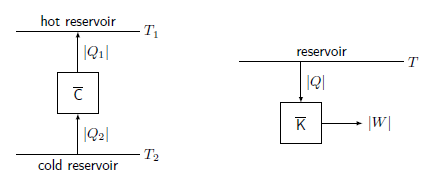
\includegraphics[scale=0.8]{secondlaw1.PNG}
    \caption{Clausius and Kelvin Engine. \cite{blundell2010concepts}}
\end{figure}
\begin{thm}
The Kelvin and Clausius statements of the Second Law of Thermodynamics are equivalent.
\end{thm}
\begin{proof}
We first show that if Clausius statement is not true, then it implies that Kelvin statement is not true. Suppose there exists a Clausius-violating device (accepts $|Q_2|$ heat from cold reservoir and dump the exact same amount to the hotter reservoir), that acts together with a heat engine (accepts heat $|Q_1|-|Q_2|$ from a single heat reservoir at temperature $T_1$ and converting it entirely into work $|W|=|Q_1|-|Q_2|$). This combined system violates Kelvin's statement since the heat accepted from the hotter reservoir is completely converted to work.\\[5pt]
Conversely, suppose there exists a Kelvin-violating device (converting heat $|Q_1'|$ entirely into work $|W|$), that acts together with a refrigerator, accepts heat $|Q_2|$ from a colder reservoir at temperature $T_2$ and transfer heat $|Q_1|$ to a hotter reservoir at temperature $T_1$. The combined system violates Clausius' statement since it takes heat $|Q_2|$ from a colder reservoir and dumps heat $|Q_2|=|Q_1|-|Q_1'|>0$ onto a hotter reservoir.
\end{proof}
\begin{figure}[H]
    \centering
    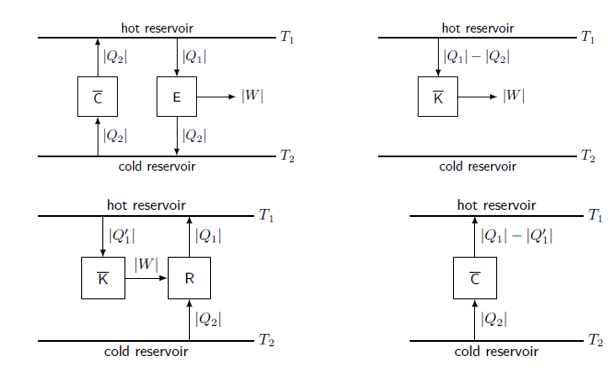
\includegraphics[scale=0.8]{secondlaw2.PNG}
    \caption{(Top) First part of proof. (Bottom) Second part of proof. \cite{blundell2010concepts}}
\end{figure}
\begin{defi}[Carnot Engine]
Carnot engine is an idealized system that is cyclic and reversible with all of its heat exchanges taking place at a hotter reservoir at temperature $T_1$ and a colder reservoir at temperature $T_2$.
\end{defi}
\begin{defi}[Ideal Refrigerator]
An ideal refrigerator is a Carnot cycle run in reverse.
\end{defi}
\begin{defi}[Carnot Cycle]
Carnot Cycle consists of 4 processes:
\begin{enumerate}
    \item A to B: isothermal expansion at $T_1$
    \item B to C: adiabatic expansion to $T_2$
    \item C to D: isothermal compression at $T_2$
    \item D to A: adiabatic compression to $T_1$.
\end{enumerate}
\begin{center}
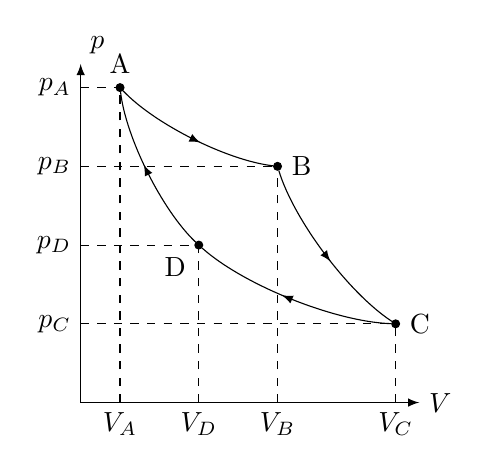
\begin{tikzpicture}[
  > = latex,
  dot/.style = {draw,fill,circle,inner sep=1pt},
  arrow inside/.style = {postaction=decorate,decoration={markings,mark=at position .55 with \arrow{>}}}
  ]
  \draw[<->] (0,4.3) node[above right] {$p$} |- (4.3,0) node[right] {$V$};
  \node[dot,label={above:A}] (@1) at (0.5,4) {};
  \node[dot,label={right:B}] (@2) at (2.5,3) {};
  \node[dot,label={right:C}] (@3) at (4,1) {};
  \node[dot,label={below left:D}] (@4) at (1.5,2) {};
  \draw[arrow inside] (@1) to[looseness=.7,bend right=20] (@2);
  \draw[arrow inside] (@2) to[looseness=.7,bend right=20] (@3);
  \draw[arrow inside] (@3) to[looseness=.7,bend left=20] (@4);
  \draw[arrow inside] (@4) to[looseness=.7,bend left=20] (@1);
  \draw[dashed,thin] (0,4) node[left] {$p_A$} -- (0.5,4);
  \draw[dashed,thin] (0.5,0) node[below] {$V_A$} -- (0.5,4);
  \draw[dashed,thin] (0,3) node[left] {$p_B$} -- (2.5,3);
  \draw[dashed,thin] (2.5,0) node[below] {$V_B$} -- (2.5,3);
  \draw[dashed,thin] (0,1) node[left] {$p_C$} -- (4,1);
  \draw[dashed,thin] (4,0) node[below] {$V_C$} -- (4,1);
  \draw[dashed,thin] (0,2) node[left] {$p_D$} -- (1.5,2);
  \draw[dashed,thin] (1.5,0) node[below] {$V_D$} -- (1.5,2);
\end{tikzpicture}
\end{center}
\end{defi}
\begin{thm}
The energy efficiency of Carnot engine with ideal gas as a working substance is $$\eta=1-\frac{T_2}{T_1}$$
\end{thm}
\begin{proof}
Since A to B is an isothermal expansion, C to D is an isothermal compression, then we have
$$|Q_{in}|=Q_{A\rightarrow B}=nRT_1\log(V_B/V_A)$$
$$|Q_{out}|=-Q_{C\rightarrow D}=-nRT_2\log(V_D/V_C)$$
Then the efficiency is $\eta=1-\frac{|Q_{out}|}{|Q_{in}|}=1-\frac{T_2}{T_1}\frac{\log(V_D/V_C)}{\log(V_A/V_B)}$. Since $TV^{\gamma-1}$ is a constant for adiabatic processes, then $V_C/V_B=V_D/V_A$ and so $\eta=1-\frac{T_2}{T_1}$.
\end{proof}
\begin{cor}
For Carnot engine, $\frac{|Q_{out}|}{|Q_{in}|}=\frac{T_2}{T_1}$
\end{cor}
\begin{thm}[Carnot's Theorem]
No engine operating between two reservoirs can be more efficient than a Carnot engine operating between the same two reservoirs.
\end{thm}
\begin{proof}
Suppose we have a hypothetical super-efficient engine SE and Carnot refrigerator CR, such that $\eta_{SE}>\eta_{CR}\implies|Q_1|>|Q_1'|$ and hence $W=|Q_1'|-|Q_2'|=|Q_1|-|Q_2|$ and hence $|Q_1|-|Q_1'|>0$ is the amount of heat dumped into the hotter reservoir while $|Q_2|-|Q_2'|>0$ is the amount of heat extracted from the colder reservoir. This violates Clausius statement.
\end{proof}
\begin{cor}
All Carnot engines operating between the same two reservoirs have the same efficiency.
\end{cor}
\begin{proof}
Prove this by setting up $\eta_1\leq\eta_2$ and $\eta_2\leq\eta_1$ and pay attention to Carnot's Theorem and Clausius' statement.
\end{proof}
\begin{figure}[H]
    \centering
    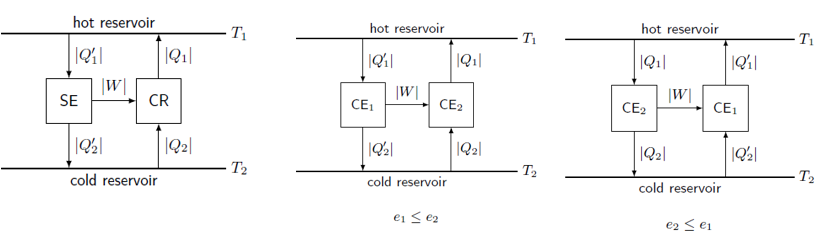
\includegraphics[scale=0.7]{secondlaw3.PNG}
    \caption{(left) Demonstrates Carnot's Theorem. (centre and right) for Corollary. \cite{blundell2010concepts}}
\end{figure}
\begin{defi}[Empirical Temperature]
Carnot's theorem means that the ratio of the heat transfers into and out of the hot and cold reservoirs is a function of the temperature of the reservoirs only. It is thus imperative to define an empirical temperature to be the ratio of heat transfers, i.e. $\frac{Q_2}{Q_1}=f(T_1,T_2)$ where $Q_1$ is heat supplied to the cold reservoir $T_1$ and $Q_2$ is heat extracted from the hot reservoir $T_2$.
\end{defi}
\begin{thm}[Clausius Inequality]
For a general cycle, reversible or not, the following relation is true
$$\oint\frac{dQ}{T}\leq 0$$
\end{thm}
\begin{proof}
Suppose heat $\delta Q_i$ at each point of a general cycle is supplied via a Carnot engine, which is connected between a common (all Carnot engines on this cycle) reservoir at temperature $T$ and the reservoir at temperature $T_i$. Each Carnot engine produces work $\delta W_i$ and for a Carnot engine, we know from Carnot's theorem that $\frac{\delta Q_i}{T_i}=\frac{\delta Q_i+\delta W_i}{T}$. The total work extracted from the cycle is $\Delta W=\sum_{i\in\text{cycle}}\delta Q_i$. And from Kelvin's statement (we cannot extract work from this assembly), the total work produced per cycle is:
$$\Delta W+\sum_{i\in\text{cycle}}\delta W_i\leq 0\implies\sum_{i\in\text{cycle}}\delta Q_i+\sum_{i\in\text{cycle}}\delta Q_i\bigg(\frac{T}{T_i}-1\bigg)\leq0\implies \sum_{i\in\text{cycle}}\frac{\delta Q_i}{T_i}\leq 0$$
where $T>0$. Changing the sum to a closed loop path integral, we obtain the Clausius' inequality.
\end{proof}
\begin{cor}
For reversible cycle, $\oint\frac{dQ}{T}=0$.
\end{cor}
\begin{defi}[Entropy]
Entropy, denoted as $S$, is $$dS=\frac{\delta q_{rev}}{T}$$ where $\delta q_{rev}$ is an infinitesimal amount of heat absorbed in a reversible process. 
\end{defi}
\begin{thm}[Second Law of Thermodynamics]
An equivalent statement of the Second Law of Thermodynamics states that for a thermally isolated system,
$$dS\geq0$$
In particular, $dS=0$ for a reversible process and $dS>0$ for an irreversible process.
\end{thm}
\begin{proof}
Consider a loop which contains an irreversible section A to B and a reversible section B to A. By Clausius' inequality, we have
$$dS=\frac{\delta q_{rev}}{T}\geq\frac{\delta q}{T}$$
For a thermally isolated system, we have $\delta q=0$. So, $dS\geq0$ in general.
\end{proof}
\begin{defi}[Entropy Change of Surroundings and System]
Since the surroundings (i.e. a heat reservoir) is much larger than the system, the temperature of the surroundings does not change, despite the heat transfer. This heat transfer, as seen from the point of view of the surroundings, is reversible, hence $\Delta q_{\text{surr}}=\Delta q_{\text{surr,rev}}$. Moreover, since energy is conserved, $\Delta q_{\text{surr}}=-\Delta q_{\text{sys}}$
$$\Delta S_{\text{surr}}:=\frac{\Delta q_{\text{surr,rev}}}{T_{\text{surr}}}=\frac{\Delta q_{\text{surr}}}{T_{\text{surr}}}=\frac{-\Delta q_{\text{sys}}}{T_{\text{surr}}}$$
As for the system, from the definition of entropy:
$$\Delta S_{\text{sys}}=\frac{q_{\text{rev,sys}}}{T}$$
This is true for both reversible and irreversible process.
\end{defi}
\begin{defi}[Equilibrium]
A system is said to be in equilibrium if $dS_{\text{univ}}=0$.
\end{defi}
\begin{defi}[Spontaneity]
A spontaneous process occurs when the resultant change in entropy of the Universe is positive, i.e. $dS_{\text{univ}}>0$. Note that
$$\Delta S_{\text{univ}}=\Delta S_{\text{surr}}+\Delta S_{\text{sys}}$$
\end{defi}
\begin{Note}[Reversible Expansion Versus Irreversible Expansion]
In general, expansion occurs when $p_{\text{internal}}>p_{\text{external}}$. Whenever there is a constant external pressure imposed on the system of gas, the expansion is said to be irreversible. It is also known as Joule expansion. It is spontaneous and system will tend towards mechanical equilibrium where $p_{\text{internal}}=p_{\text{external}}$.\\[5pt]
In contrast, for a reversible expansion, the external pressure is infinitesimally greater than the internal pressure. Any infinitesimal change in the external pressure will thus change the direction of the process. Such a process is infinitely slow since it is at equilibrium.
\end{Note}
\begin{defi}[Entropy]
We can also define the entropy of a system, $S=S(E)$, to be 
$$S(E)=\log(\Omega(E))$$
where $\Omega(E)$ is the number of states with energy $E$.
\end{defi}
\begin{defi}[Thermodynamic Temperature]
The thermodynamic temperature $T$ of a system with entropy function $S(E)$ is
$$\frac{1}{T}:=\frac{dS(E)}{dE}$$
\end{defi}
\begin{Note}[Maximal entropy at equilibrium]
Consider an isolated system, partitioned into systems 1 and 2 which are in thermal contact with each other. The subsystems have energies $E_1$ and $E_2$ respectively. The total energy is $E=E_1+E_2$, which is conserved even after the isolated systems come into contact. The number of available states is
$$\Omega(E_1,E_2)=\Omega_1(E_1)\Omega_2(E_2)=e^{S_1(E_1)}e^{S_2(E_2)}\implies S(E_1,E_2)=S_1(E_1)+S_2(E_2)=S_1(E_1)+S_2(E-E_1)$$
so thermal contact allows $E_1$ to take on any value that state 1 allows, i.e. $E_1^i$ for all possible states labelled by $i$. The number of available states given fixed energy $E$ is $$\Omega(E)=\sum_i\exp(S_1(E_1^i)+S_2(E-E_1^i))$$ which will have an extremely high and narrow maximum at a particular energy value, say $E_1$. Thus, the sum dominates at this value $E_1$, thus maximizing the entropy $S$.
$$\frac{dS}{dE_1}=\frac{dS_1}{dE_1}+\frac{dS_2}{dE_2}\frac{dE_2}{dE_1}=0$$
with $E_2=E-E_1$, so $\frac{dS_1}{dE_1}-\frac{dS_2}{dE_2}=\frac{1}{T_1}-\frac{1}{T_2}=0$ at equilibrium energy $E_1$. Thus, $T_1=T_2$. The condition for the maximum of $S$ is
$$\frac{d^2S}{dE_1^2}=\frac{d^2}{dE_1^2}(S_1(E_1)+S_2(E-E_1))=\frac{d}{dE_1}\bigg(\frac{1}{T_1}-\frac{1}{T_2}\bigg)=-\frac{1}{T_1^2}\frac{dT_1}{dE_1}-\frac{1}{T_2^2}\frac{dT_2}{dE_2}$$
where $E_2=E-E_1$. At equilibrium, $T_2=T_1$, so
$$\frac{d^2S}{dE_1^2}=-\frac{1}{T_1^2}\bigg(\frac{dT_1}{dE_1}+\frac{dT_2}{dE_2}\bigg)$$
For maximum $S$, we require
$$\frac{dT_1}{dE_1}+\frac{dT_2}{dE_2}>0$$
This will work if $\frac{dT}{dE}>0$ for every system, i.e. energy increases with temperature. In another words, the slope of $S(E)$ decreases with energy $E$. 
\end{Note}
\subsection{Chemical Potential}
\begin{defi}[Chemical Potential]
The chemical potential $\mu$ is the reversible rate of change of internal energy caused by changing mole number $n$.
\end{defi}
\begin{thm}
Gradient in chemical potential influences particle exchange.
\end{thm}
\begin{proof}
We have $dU=TdS-pdV+\mu dN\implies dS=\frac{dU}{T}+\frac{pdV}{T}-\frac{\mu dN}{T}$. Writing $dS=(\frac{\partial S}{\partial U})_{N,V}dU+(\frac{\partial S}{\partial V})_{N,U}dV+(\frac{\partial S}{\partial N})_{U,V}dN$ and by comparison, we get $(\frac{\partial S}{\partial N})_{U,V}=-\mu/T$. Consider two systems which are able to exchange particles with each other, but remain isolated from their surroundings. If system 1 loses $dN$ particles, system 2 must gain $dN$ particles and so $dS=(\frac{\mu_1}{T_1}-\frac{\mu_2}{T_2})dN\geq0$. Assuming $T_1=T_2$, we find $dN>0$ when $\mu_1>\mu_2$.
\end{proof}
\begin{Note}[Internal Energy as Extensive Function]
Since internal energy is extensive, i.e. depends linearly on the size of the system, then $U(\lambda S, \lambda X)$, where $X$ are all other possible extensive variables (could be generalized). Then, $U(\lambda S,\lambda X)=\lambda U(S,X)$. Thus, $U(S,X)$ is a first-order homogeneous function of $S$ and $X$.
\end{Note}
\begin{thm}[Gibbs-Duhem Equation]
The Gibbs-Duhem equation, in the energy representation, is
$$0=SdT+\sum_{i=1}^rx_idF_i+\sum_{i=1}^rN_id\mu_i$$
where only $r+s$ variables are independent. It states that adjacent equilibrium states cannot differ only in one of these independent variables.
\end{thm}
\begin{proof}
We invoke Euler's theorem for first-order homogeneous functions which are $f(\{u_i\})=\lambda f(\{x_i\})$ where $u_i=\lambda x_i$ $\forall i\in[1,n]$. Then, $(\frac{\partial f(\{u_i\})}{\partial \lambda})_{x_i}=f(\{x_i\})$ but $df(\{u_i\})=\sum_{s=1}^n(\frac{\partial f}{\partial u_s})_{u_k}du_s$ and so
$$\bigg(\frac{\partial f}{\partial\lambda}\bigg)_{x_i}=\sum_{i=1}^n\bigg(\frac{\partial f}{\partial u_i}\bigg)_{u_i}\bigg(\frac{\partial u_i}{\partial\lambda}\bigg)_{x_i}=\sum_{i=1}^n\bigg(\frac{\partial f}{\partial u_i}\bigg)_{u_j}x_i$$
This implies $f(\{x_i\})=\sum_{i=1}^n(\frac{\partial f}{\partial u_i})_{u_j}x_i$ is true for all $\lambda$. Take $\lambda=1$, then $f(\{x_i\})=\sum_{i=1}^n(\frac{\partial f}{\partial x_i})_{x_j}x_i$. Since $U(S,X)$ is first-order homogeneous, by Euler's theorem, we have $U=TS+Fx+\mu N\implies dU=TdS+SdT+\sum_{i=1}^r(x_idF_i+F_idx_i)+\sum_{i=1}^r(\mu_idN_i+N_id\mu_i)$ but $dU=TdS+\sum_{i=1}^rF_idx_i+\sum_{i=1}^r\mu_idN_i$ and so we recover the desired equation.
\end{proof}
\begin{cor}
$$U=TS-PV+\mu N$$
\end{cor}
\begin{proof}
Follows from Euler's theorem.
\end{proof}
\begin{prop}
For a reversible chemical reaction, we must have $\sum_i\nu_i\mu_i=0$.
\end{prop}
\begin{proof}
By Gibbs-Duhem equation, we have $d\mu_i=-s_idT+v_idp$. The change in chemical potential is thus zero at constant $T$ and $P$. The variation of $G$ about the equilibrium ratio of chemical components satisfies
$$dG=\sum_i\mu_idN_i=0$$
But the $dN_i$'s are related by matter conservation, so $dN_i/\nu_i$ is a constant. We then have 
$$\sum_i\nu_i\mu_i=0$$
where $\nu_i$'s are the ratios, with $\nu>0$ for reactants and $\nu<0$ for products. 
\end{proof}
\begin{defi}[Equilibrium constant for concentration]
$$K_c(T):=\prod_ic_i^{\nu_i}$$
\end{defi}
\begin{prop}
$$\ln K_c(T)=-\frac{1}{k_BT}\sum_i\nu_i\mu_{0,i}(T,P)$$
\end{prop}
\begin{proof}
Combining $\sum_i\nu_i\mu_i=0$ and $\mu_i(P_i,T)=\mu_{0,i}(P,T)+k_BT\ln c_i$, we have
$$0=\sum_i\nu_i\mu_{0,i}+k_BT\sum_i\nu_i\ln c_i=\sum_i\nu_i\mu_{0,i}+k_BT\ln\prod_i c_i^{\nu_i}$$
Hence, $\ln K_c(T)=-\frac{1}{k_BT}\sum_i\nu_i\mu_{0,i}(T,P)$.
\end{proof}
\newpage
\subsection{Potentials and Availability}
\subsubsection*{Availability}
\begin{prop}
Maximizing the total entropy of system and reservoir $R$ with respect to the state of the system is equivalent to minimizing the availability of the system.
\end{prop}
\begin{proof}
From the principle of maximum entropy, we have
$$0\leq dS_{\text{tot}}=dS+dS_R=dS+dS_R=dS+\frac{dU_R+P_RdV_R-\mu_RdN_R}{T_R}$$
Maximize $S_{\text{tot}}$ is thus equivalent to maximizing the quantity
$$\int(T_RdS-dU-P_RdV+\mu_RdN)=\int(d(T_RS)-dU-d(P_RV)+d(\mu_RN))=T_RS-U-P_RV+\mu_RN$$
We denote this quantity to be the availability $-A$. The reason for the minus sign is apparent later.
\end{proof}
\begin{remarks}
The change in availability is written in terms of its natural variables $S$, $V$ and $N$:
$$dA=dU-T_RdS+P_RdV-\mu_RdN=(T-T_R)dS-(P-P_R)dV+(\mu-\mu_R)dN$$
\end{remarks}
\begin{prop}
The availability is the maximum useful work possible during a process that brings the system into equilibrium with a reservoir $R$, upon contact.
\end{prop}
\begin{proof}
The total work extracted is
\begin{align}
-dW&=dU+dU_R\nonumber\\&=d(A+T_RS-P_RV+\mu_RN)+T_RdS_R-P_RdV_R+\mu_RdN_R\nonumber\\&=dA+T_RdS+T_RdS_R-P_RdV+P_RdV+\mu_RdN-\mu_RdN\nonumber\\&=dA+T_Rd(S+S_R)\nonumber
\end{align}
But since $d(S+S_R)\geq0$, we have $-dW\geq dA$. The maximum work is attained when $S+S_R$ stays constant.
\end{proof}
\begin{cor}
The availability of a system in equilibrium with a reservoir is always zero.
\end{cor}
\begin{proof}
The availability is defined to be the extractable work on attaining equilibrium. This is zero if the system is already in equilibrium.
\end{proof}
\begin{Note}[Free energy]
Reversibly compress a monatomic ideal gas that is connected to a reservoir. The energy input is in the form of work. The temperature, and hence internal energy is constant. The work flows directly out of the system into the reservoir as heat. If we reverse this reversibly, we recover the energy back. Energy conservation needs to be applied to both the system and the reservoir. The free energy of an isothermal system is the quantity which corresponds to energy conservation in the system and the reservoir.
\end{Note}
\subsubsection*{Legendre transform}
\begin{defi}[Legendre Transformation]
A Legendre transform converts from a function of one set of variables to another function of a conjugate set of variables. 
\end{defi}
\begin{thm}
The Legendre transform of $f=f(x_1,...,x_n)$ is $g=f-\sum_{i=r+1}^nu_ix_i$, where $u_i=(\frac{\partial f}{\partial x_i})_{x_j}$, such that $g=g(x_1,...,x_r,u_{r+1},...,u_n)$ where $u_{r+1},...,u_n$ are conjugate variables to $x_{r+1},...,x_n$.
\end{thm}
\begin{proof}
We evaluate $dg$
$$dg=df-\sum_{i=r+1}^n(u_xdx_i+x_idu_i)=\sum_{i=1}^ru_idx_i+\sum_{i=r+1}^n(-x_i)du_i$$
$g$ is indeed a function of $x_i$ for $i\in[1,r]$ and $u_i$ for $i\in[r+1,n]$.
\end{proof}
\subsubsection*{Thermodynamic potentials}
\begin{defi}[Thermodynamic potentials]
Thermodynamic potentials are generated by Legendre transforms. The variables which are differentiated with respect to are the `natural variables' of the corresponding thermodynamic potential.
\end{defi}
\begin{remarks}\leavevmode
\begin{enumerate}
    \item A thermodynamic potential is minimized in equilibrium under the conditions that its natural variables are held fixed.
    \item If one knows any of the thermodynamic potentials as a function of its natural variables, one has complete thermodynamic information about the equilibrium state.
    \item The appropriate thermodynamic potential is the property of the system that reflects global energy conservation.
\end{enumerate}
\end{remarks}
\begin{eg}
Since internal energy is the sum of $\delta q$ and $\delta W$, then by the first law of thermodynamics,
$$dU=TdS-pdV$$
where $S$ and $V$ are natural variables of $U$, i.e. $U=U(S,V)=TS-PV$. We correspondingly define three more thermodynamic potentials: enthalpy $H$, Gibbs function $G$ and Helmholtz function $F$:
$$H=U+PV\implies dH=dU+d(PV)=TdS-PdV+PdV+VdP=TdS+VdP$$
$$G=H-TS\implies dG=dH-d(TS)=TdS+VdP-TdS-SdT=-SdT+VdP$$
$$F=U-TS\implies dF=dU-d(TS)=TdS-PdV-TdS-SdT=-SdT-PdV$$
The natural variables are thus $H(S,p)$, $F(T,V)$, $G(P,T)$. Note that here we take $N$ to be fixed. Otherwise, we have $F(T,V,N)$, $G(P,T,N)$, $H(S,P,N)$ and $U(S,V,N)$. Physically, they mean:
\begin{itemize}
    \item Internal Energy $U$: energy needed to create a system. To attain equilibrium at constant $V$, $S$ and $N$, we minimize $U$, i.e. $dA=dU$.
    \item Enthalpy $H$: energy needed to create a system plus the work needed to make room for it. To attain equilibrium at constant $P$, $S$ and $N$, we minimize $H$, i.e. $dA=dU+PdV=d(U+PV)=dH$.
    \item Gibbs Free Energy $G$: energy needed to create a system and make room for it minus the energy you can get from the environment. To attain equilibrium at constant $T$, $P$ and $N$, we minimize $G$, i.e. $dA=dU-TdS+PdV=d(U-TS+PV)=dG$.
    \item Helmholtz Free Energy $F$: energy needed to create a system minus the energy you can get from the environment. To attain equilibrium at constant $T$, $V$ and $N$, we minimize $F$, i.e. $dA=dU-TdS=d(U-TS)=dF$.
\end{itemize}
One last possible thermodynamic potential is the grand potential $\Phi(T,V,\mu)=F-\mu N$. To attain equilibrium at constant $T$, $V$ and $\mu$, we minimize $\Phi$.
\end{eg}
\begin{remarks}
For $G$, the only extensive natural variable is $N$, so from Euler's Theorem, we can write $G=U-TS+PV=\mu N$. Similarly, since the only extensive natural variable for $\Phi$ is $V$, we can write $\Phi=U-TS-\mu N=-PV$.
\end{remarks}
\begin{cor}
The thermodynamic potentials can indeed be inter-converted from Legendre Transformation.
\end{cor}
\begin{proof}
Since $T=(\frac{\partial U}{\partial S})_V$ and $P=-(\frac{\partial U}{\partial V})_S$, then $(T,S)$ and $(P,-V)$ are conjugate variables pair. To construct $F$ from $U$, we subtract the quantity $S$ times the variable conjugate to $S$, which is $T$, i.e. $F=U-TS$. Similarly, to construct $H$ from $U$, we subtract the quantity $V$ with its conjugate, which is $-P$, i.e. $H=U-(-PV)$. Lastly, to construct $G$ from $U$, we first convert it to $F$ and then deduct $-PV$. 
\end{proof}
\begin{thm}[Maxwell's Relations]
$$\bigg(\frac{\partial T}{\partial V}\bigg)_S=-\bigg(\frac{\partial p}{\partial S}\bigg)_V,\quad\bigg(\frac{\partial T}{\partial p}\bigg)_S=-\bigg(\frac{\partial V}{\partial S}\bigg)_p,\quad\bigg(\frac{\partial p}{\partial T}\bigg)_V=-\bigg(\frac{\partial S}{\partial V}\bigg)_T,\quad\bigg(\frac{\partial V}{\partial T}\bigg)_p=-\bigg(\frac{\partial S}{\partial p}\bigg)_T$$
\end{thm}
\begin{proof}
For all four, we use Clairaut's theorem (symmetry of second partial derivatives). The first, second, third and fourth were obtained from $U$, $H$, $F$ and $G$ respectively.\\[5pt]
Alternatively, one may use Jacobian. Consider a cyclic process that can be described in both the T-S and p-V plane. The internal energy $U$ is a state function and therefore doesn't change in a cycle and since $\oint dU=0$, we have $\oint pdV=\oint TdS$ and so $\frac{\partial(T,S)}{\partial(p,V)}=1\implies\frac{\partial(T,S)}{\partial(x,y)}=\frac{\partial(p,V)}{\partial(x,y)}$ where $(x,y)$ can be taken as $(T,p)$, $(T,V)$, $(p,S)$ and $(S,V)$ respectively.
\end{proof}
\begin{remarks}
In general, there are more than 4 Maxwell's relations. Given a particular thermodynamic potential, expressed in terms of its $(1+r+s)$ natural variables, there are $(1+r+s)(r+s)/2$ distinct pairs of mixed second derivatives yielding $(1 + r + s)(r + s)/2$ Maxwell’s relations.
\end{remarks}
\begin{eg}
$dU$ gives the heat transfer $\delta q$ to a system at constant $V$ while $dH$ gives the heat transfer $\delta q$ to a system at constant $p$, i.e. energetics of a chemical reaction.
\end{eg}
\begin{thm}[Gibbs-Helmholtz Equations]
$$U=-T^2\bigg(\frac{\partial}{\partial T}\frac{F}{T}\bigg)_V,\quad H=-T^2\bigg(\frac{\partial}{\partial T}\frac{G}{T}\bigg)_P$$
\end{thm}
\begin{proof}
Using the expressions $S=-(\frac{\partial F}{\partial T})_V$ and $S=-(\frac{\partial G}{\partial T})_p$, we get
$$U=F+TS=F-T\bigg(\frac{\partial F}{\partial T}\bigg)_V=-T^2\bigg(\frac{\partial}{\partial T}\frac{F}{T}\bigg)_V,\quad H=G+TS=G-T\bigg(\frac{\partial G}{\partial T}\bigg)_p=-T^2\bigg(\frac{\partial}{\partial T}\frac{G}{T}\bigg)_p$$
\end{proof}
\begin{cor}
The following statements are true:
\begin{itemize}
    \item At constant entropy, i.e. reversible adiabatic change, the work done by a system is equal to $dU$.
    \item At constant temperature, the maximum amount of energy which can be converted to work is given by $-dF$.
    \item At constant temperature and pressure, the maximum amount of energy which can be converted to non-$pV$ work is given by $dG$.
\end{itemize}
\end{cor}
\begin{proof}
First one is trivial, since $dU=-pdV$. For second one, since
$$dF=\delta q_{\text{sys}}+\delta W-TdS-SdT$$
and the $\delta q_{\text{sys}}=-\delta q_{\text{res}}$, then at constant temperature (same as that of the reservoir),
$$dF=\delta W-T(dS_{\text{res}}+dS)=\delta W-TdS_{\text{total}}\implies -\delta W=-dF-TdS_{\text{total}}\leq -dF$$
The maximum amount of energy which can be converted to work, occurs when $dS_{\text{total}}=0$. For third one, since at constant temperature and pressure,
$$dG=\delta q_{sys}+\delta W+pdV−TdS$$
when the change is reversible, $\delta q_{sys}=TdS$. Furthermore, $\delta W=-pdV+\delta W_{nonPV}$ and so $\delta G=\delta W_{nonpV}$ and this maximum conversion occurs in a reversible process.
\end{proof}
\begin{eg}
$G$ is extensively used by chemists since it involves constant temperature and pressure. But yet $F$ is extensively used by physicists since in statistical mechanics, $F$ is easier to evaluate. Both allow us to find the entropy change of the surroundings in terms of the properties of the system.
\end{eg}
\newpage
\subsection{Phase Transitions}
\begin{defi}[Phase transition]
A phase of a thermodynamic system and the states of matter have uniform physical properties. During a phase transition of a given medium, certain properties of the medium change, often discontinuously, as a result of the change of external conditions, such as temperature, pressure, or others.
\end{defi}
\begin{remarks}\leavevmode
\begin{enumerate}
    \item At a given temperature and pressure, the stable phase will be the one with lower Gibbs free energy.
    \item The condition for phase equilibrium: the chemical potential $\mu$ of both phases are equal.
    \item Recall Gibbs-Duhem relation $d\mu=-sdT+vdP$ where $s$ and $v$ are the entropy and volume per particle respectively. At high temperatures, the phase with highest $s$ have the smallest $\mu$, so more stable since $(\frac{\partial\mu}{\partial T})_p=-\frac{S}{N}=s$. At high pressures, the phase with smallest $v$ have the smallest $\mu$, so more stable since $(\frac{\partial\mu}{\partial p})_T=\frac{V}{N}=v$. 
\end{enumerate}
\end{remarks}
\begin{thm}[Clausius-Clapeyron relation]
The Clausius–Clapeyron relation is a way of characterizing a discontinuous phase transition (involving a latent heat, with no change in temperature) between two phases of matter of a single constituent. The gradient of the phase boundary on the $P$-$T$ plane is
$$\frac{dP}{dT}=\frac{L}{T(V_2-V_1)}$$
\end{thm}
\begin{proof}
Suppose $N_1$ particles of phase 1 are in equilibrium with $N_2$ particles of phase 2. The total Gibbs free energy is $G_{tot}=N_1\mu_1+N_2\mu_2$. In phase equilibrium, $dG_{tot}=0\implies\mu_1=\mu_2$. At a given temperature and pressure, each coexisting phase has the same chemical potential. We can thus characterize the line of coexistence of two phases to be $\mu_1(P,T)=\mu_2(P,T)$. Along this phase boundary, we have $\mu_1(P+dP,T+dT)=\mu_2(P+dP,T+dT)\implies d\mu_1=d\mu_2\implies -s_1dT+v_1dP=-s_2dT+v_2dP$, where $s$ and $v$ are entropy and volume per particle respectively. We then have 
$$\frac{dP}{dT}=\frac{(S_2-S_1)}{(V_2-V_1)}=\frac{L}{T(V_2-V_1)}$$
where $L=T(S_2-S_1)$ is the latent heat evolved from the phase transition.
\end{proof}
\begin{defi}[Triple Point]
In thermodynamics, the triple point of a substance is the temperature and pressure at which the three phases (gas, liquid, and solid) of that substance coexist in thermodynamic equilibrium.
\end{defi}
\begin{defi}[Critical Point]
In thermodynamics, a critical point is the end point of a phase equilibrium curve. At the critical point, defined by a critical temperature $T_c$ and a critical pressure $P_c$, phase boundaries vanish. One example is the Curie temperature for paramagnets, where $T>T_c$, there is no clear boundary between magnetized up and magnetized down.
\end{defi}
\begin{remarks}
It is common to describe various equilibrium states by P-V diagram, where one follows curves of constant entropy (adiabatic changes) or curves of constant temperature (isothermal changes) as they correspond to the system adiabatically isolated or in contact with a heat bath respectively. A phase transition appears as a jump in an isothermal curve. For the isothermal curve of the molar free energy, the slope of one phase is equal the slope of the other (joined by a common straight tangential line).
\end{remarks}
\begin{Note}[Phase Transition Curves]
A phase transition appears as a jump in an isothermal curve. $(T,P(T))$ is a point on the coexistence line, such that $P(T)$ is a solution to the Clausius-Clapeyron equation. $v^{(1)}(T)$ and $v^{(2)}(T)$ are the molar volumes of the two phases with $\Delta v(T)$ being the difference. Where the isothermal curve is continuous within one phase, it has a negative slope since $(\frac{\partial P}{\partial V})_T<0$ in stable equilibrium. Since $v^{(2)}<v^{(1)}$, the phase 1 is gaseous while phase 2 is liquid. Pressure is derived from free energy, i.e. $P=-\frac{\partial F}{\partial V}$. So
$$F(T,V,n)=nF\bigg(T,\frac{V}{n},1\bigg)=nf(T,V)\implies P=-\bigg(\frac{\partial f}{\partial v}\bigg)_T=P(T,V)$$
We have $-(\frac{\partial f^{(1)}}{\partial v})_T=-(\frac{\partial f^{(2)}}{\partial v})_T$ holds for $(T,P(T))$ on the coexistence line for phases 1 and 2. On this line, we also have equal chemical potentials, i.e. $\mu^{(1)}(T,v^{(1)})=\mu^{(2)}(T,v^{(2)})$.  The corresponding isothermal curve for molar free energy $f$, have equal slopes at the points $(v^{(2)},f^{(2)}(T,v^{(2)}))$ and $(v^{(1)},f^{(1)}(T,v^{(1)}))$. These two points can be connected by a common straight tangential line
$$f^{(2)}(T,v^{(2)})-f^{(1)}(T,v^{(1)})=-P(T)[v^{(2)}-v^{(1)}]\implies (f+Pv)^{(1)}=(f+Pv)^{(2)}$$
consistent with $\mu^{(1)}=\mu^{(2)}$. We note that the curvature of the isothermal curve has the wrong sign in some range, i.e. $(\frac{\partial^2f}{\partial v^2})_T<0$ or $(\frac{\partial P}{\partial v})_T>0$. The requirement for $\mu^{(1)}=\mu^{(2)}$ gives rise to the Maxwell construction. Since $[v^{(1)}-v^{(2)}]P(T)=f(T,v^{(2)})-f(T,v^{(1)})$, we have the two shaded areas above and below the coexistence line respectively to be the same size.
\end{Note}
\begin{figure}[H]
    \centering
    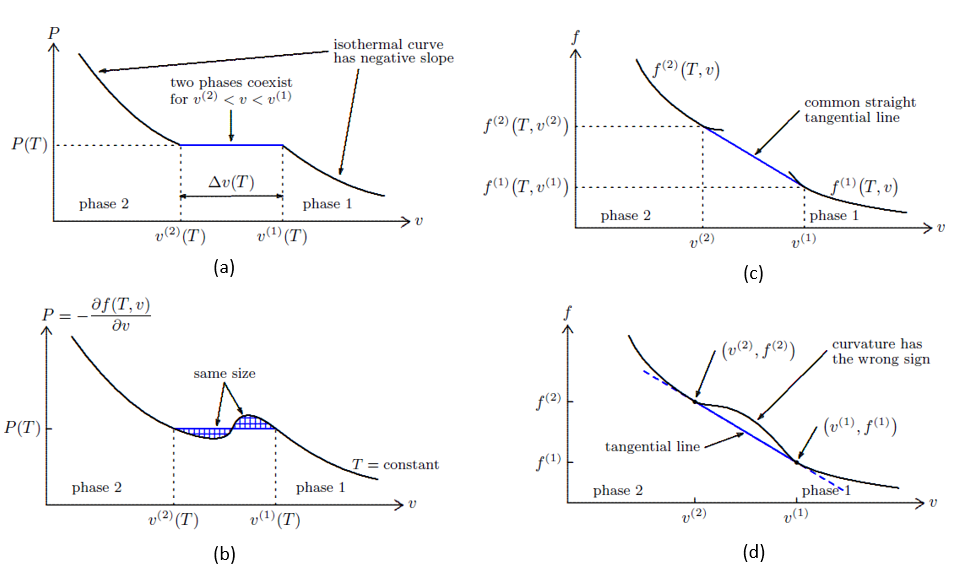
\includegraphics[width=\linewidth]{phasetransition.PNG}
    \caption{Phase Transition Curves: (a-b) P-v Curve; (c-d) f-v curve}
\end{figure}
\begin{defi}[Metastable Phases]
It is possible to warm a liquid above boiling point to form metastable superheated liquid. Similarly, it is possible to cool a vapor below boiling point to form metastable supercooled vapor.
\end{defi}
\begin{eg}
Consider a liquid with $p_{liq}$ in equilibrium with a vapor at pressure $p$, then $\mu_{liq}=\mu_{vap}$. Suppose $p_{liq}\rightarrow p_{liq}+dp_{liq}$, then $p\rightarrow p+dp$ in order to stay in equilibrium.
$$\bigg(\frac{\partial\mu_{liq}}{\partial p_{liq}}\bigg)_Tdp_{liq}=\bigg(\frac{\partial\mu_{vap}}{\partial p}\bigg)_Tdp\implies v_{liq}dp_{liq}=v_{vap}dp\implies p=p_0e^{v_{liq}\Delta p_{liq}/RT}$$
where $\Delta p_{liq}=2\gamma/r$ (surface tension). This is Kelvin's formula. So small droplets have very high vapor pressure. With the very high pressure, they can evaporate instead of growing. This high pressure stabilizes the vapour, even though it is the thermodynamically unstable phase. The thermodynamic driving force to condense is overcome by the tendency to evaporate.\\[5pt]
Similar effect occurs for superheated liquids. As you boil the liquid, any bubble of vapor which does form tends to collapse. Liquid can be kinetically stable above its boiling point, the only bubbles which then do survive are very large ones, and this causes violent bumping. This can be avoided by boiling with small pieces of glasses, providing plenty of nucleation centres for small bubbles to form. 
\end{eg}
\newpage
\begin{Note}[Phase Change in van der Waals gas]
The Helmholtz function is obtained from $p=-(\frac{\partial F}{\partial V})_T$ and so $F=-RT\log(V-b)-\frac{a}{V}+f(T)$ where $f(T)$ is a function of temperature. The Gibbs function is $G=F+pV=f(T)-RT\log(V-b)-\frac{a}{V}+pV$. $G$ is plotted for $T=0.9T_c$ (Fig \ref{vanderwaals}) and it was discovered that the Gibbs function becomes multiply valued for certain values of pressure. Since a system held at constant temperature and pressure will minimize $G$, the system will normally ignore the upper loop, i.e. path BXYB, and proceed from A to B to C as the pressure is reduced.\\[5pt]
Moreover, we see that the two points B$_1$ and B$_2$ on the curve representing the volume correspond to the single point B on the curve representing $G$. Since $G$ is the same for these two points, phases corresponding to these two points can be in equilibrium with each other. Liquid is stable in the region AB and gas is stable in the region BC. The line BX represents metastable superheated liquid while the line BY represents metastable supercooled gas. We note that the triangle BXY vanishes for $T>T_c$. When $T>T_c$, the sharp distinction between liquid and gas is lost.
\end{Note}
The van der Waals isotherms are as follow: with red ($T=T_c$), blue ($T>T_c$) and black ($T<T_c$).
\begin{center}
\begin{tikzpicture}
      \draw[->] (0,0) -- (6,0) node[right] {$V$};
      \draw[->] (0,-1) -- (0,4) node[left] {$p$};
      \draw [dashed] (1,0) -- (1,3);
      \draw[domain=0.44:5,smooth,variable=\x,black] plot ({\x},{8*0.8/(3*\x-1)-(3/\x^2))});
      \draw[domain=0.6:5,smooth,variable=\x,red] plot ({\x},{8*1.2/(3*\x-1)-(3/\x^2))});
      \draw[domain=1.2:5,smooth,variable=\x,blue] plot ({\x},{8*2/(3*\x-1)-(3/\x^2))});
      \draw (0,0) node[left]{0};
      \draw (1,0) node[below]{$V_c$};
\end{tikzpicture}
\end{center}
\begin{thm}[Maxwell Construction]
Phase existence occurs between two points, when the two areas bounded by the isotherm are equal.
\end{thm}
\begin{proof}
We have $(\frac{\partial G}{\partial p})_T=V$ and so $G(p_1,T)=G(p_2,T)+\int_{p_2}^{p_1}Vdp$. Since $G(p_{B_1},T)=G(p_{B_2},T)$, we have $\int_{p_{B_1}}^{p_{B_2}}Vdp=0$. This represents the shaded areas.
\end{proof}
\begin{figure}[H]
    \centering
    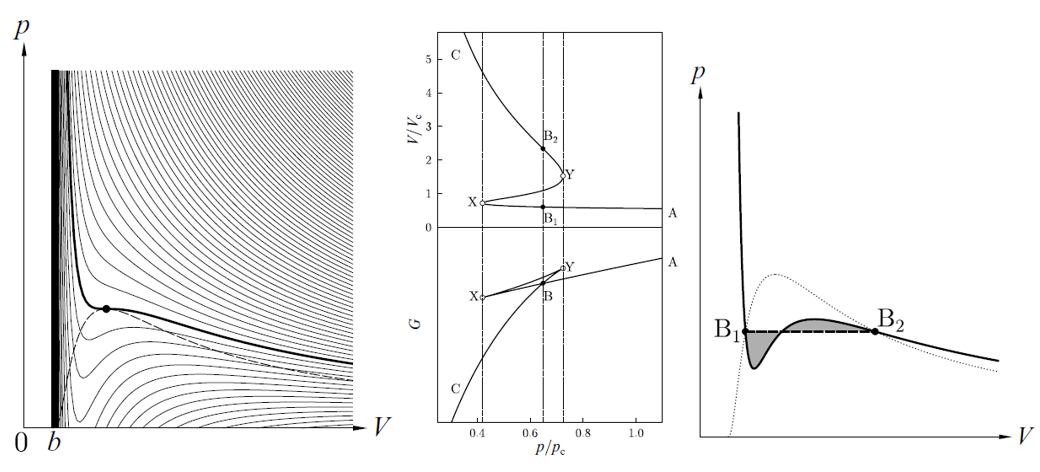
\includegraphics[width=\linewidth]{vanderwaals.PNG}
    \caption{(left) van der Waals Isotherms (thin lines) with the critical isotherm (thick line) and region in which liquid and vapor are in equilibrium (dashed line) and the critical point; (centre) Behaviour of $V$ and $G$ of a van der Waals gas as a function of $p$ at $T=0.9T_c$; (right) Maxwell construction for van der Waals gas, phase existence occurs between points B$_1$ and B$_2$ when the shaded areas are equal.}
    \label{vanderwaals}
\end{figure}
\newpage
\subsection{Ideal gas mixtures}
In a mixture of non-interacting ideal gases, the property of the mixture is just the sum of the independent contributions of each species of `component' of gas. 
\begin{thm}[Dalton's law]
The total pressure is the sum of the partial pressures, i.e. $p=\sum_ip_i=N_ik_BT/V$, where the entire mixture is at temperature $T$ and volume $V$.
\end{thm}
\begin{prop}[Entropy of mixing]
The difference between the entropy of an ideal gas mixture and that of a separated out assembly of pure gases each at pressure $p$ is called the entropy of mixing, and it is
$$\Delta S=-Nk_B\sum_i(p_i/p)\log(p_i/p)$$
\end{prop}
\begin{proof}
From first law,
$$dS=\frac{dU}{T}+\frac{pdV}{T}\implies S=C_V\log T+Nk_B\log V$$
unique up to some constant. But, $T$ and $V$ are the same for the entire mixture, so we express it in terms of partial pressures (intensive variables), to get
$$S=C_p\log T-Nk_B\log p$$
Starting with a collection of vessels all at the same pressure $p$ and containing numbers of particles $N_i$ of gas component $i$, we could achieve the mixing process by first, an isothermal expansion of each component $i$ to the desired final pressure $p_i$, followed by joining together all the containers, then isothermally compressing again to the same pressure $p$ to partial pressure $p_i$, its entropy changes by $\Delta S_i=-N_ik_B\log(p_i/p)$. The difference is entropy is
$$\Delta S=-k_B\sum_iN_i\log(p_i/p)=-Nk_B\sum_ic_i\log c_i$$
where $c_i=N_i/N=p_i/p$ is the concentration of the $i$th component.
\end{proof}
\begin{prop}
The chemical potential of the $i$th component, which is present with concentration $c_i$ in a mixture of ideal gases, differs from the chemical potential for the pure gas at the same total pressure by $k_BT\log c_i$. 
\end{prop}
\begin{proof}
At constant $T$, we have
$$\bigg(\frac{\partial G}{\partial p}\bigg)_T=\bigg(\frac{\partial\mu N}{\partial p}\bigg)_T=\frac{k_BTN}{p}\implies\mu (T,p)=\mu(T,p_0)+k_BT\log\frac{p}{p_0}$$
The Gibbs free energy of the mixture is $G=\sum_iG_i$. Using $(\partial G_i/\partial p_i)_{T,N_i}=V$, we have
$$G_i(p_i,T)=G_i(p,T)+\int_p^{p_i}Vdp=G_i(p,T)+N_ik_BT\log c_i$$
Since $G_i=\mu_iN_i$, we have $\mu_i(p_i,T)=\mu_{0,i}(p,T)+k_BT\log c_i$. 
\end{proof}
\begin{eg}
For a chemical equilibrium, we start with ensuring the Gibbs free energy is a minimum. At constant $T$ and $p$, $d\mu_i=0$ from Gibbs-Duhem equation. A variation of $G$ about the equilibrium ratio of chemical components thus satisfy
$$0=dG=\sum_i\mu_idN_i=\sum_i\nu_i\mu_i$$
where the $dN_i$;s are related by matter conservation. Now, with the equation for $\mu_i$, we have
$$0=\sum_i\nu_i\mu_{0,i}+k_BT\sum_i\nu_i\log c_i=\sum_i\nu_i\mu_{0,i}+k_BT\log\prod_i c_i^{\nu_i}$$
We can define the equilibrium constant for concentration to be $K_c(T)=\prod_i c_i^{\nu_i}$.
\end{eg}
\newpage
\section{Recap of Statistical Mechanics}
\subsection{Definitions}
\begin{Note}[Idea of Statistical Mechanics]
The primary goal of statistical thermodynamics (also known as equilibrium statistical mechanics) is to derive the classical thermodynamics of materials in terms of the properties of their constituent particles and the interactions between them. Physical properties of thermodynamic systems in equilibrium are given by the averages calculated with an appropriate ensemble which assign probabilities to respective microstates. Whereas statistical mechanics proper involves dynamics, here the attention is focused on statistical equilibrium (steady state). Statistical equilibrium does not mean that the particles have stopped moving (mechanical equilibrium), rather, only that the ensemble is not evolving.
\end{Note}
\begin{Note}[Fundamental Postulate of Statistical Mechanics]
The fundamental postulate is the \emph{equal a priori probability postulate} which states that:\\[5pt]
\emph{For an isolated system with an exactly known energy and exactly known composition, the system can be found with equal probability in any microstate consistent with that knowledge.}\\[5pt]
There are various arguments in favour of the equal a priori probability postulate:
\begin{itemize}
    \item Ergodic hypothesis: An ergodic system is one that evolves over time to explore all accessible states: all those with the same energy and composition. In an ergodic system, the microcanonical ensemble is the only possible equilibrium ensemble with fixed energy. This approach has limited applicability, since most systems are not ergodic.
    \item Principle of indifference: In the absence of any further information, we can only assign equal probabilities to each compatible situation.
    \item Maximum information entropy: A more elaborate version of the principle of indifference states that the correct ensemble is the ensemble that is compatible with the known information and that has the largest Gibbs entropy (information entropy).
\end{itemize}
\end{Note}
\begin{defi}[Ensemble]
An ensemble is a mental collection of identical copies of the same physical system in which each copy is in a different microstate labelled by $\alpha$.
\end{defi}
\begin{defi}[Ensemble Average]
Ensemble average of the physical property $X$ is $\langle X\rangle=\sum_\alpha p_\alpha X_\alpha$ for $0\leq p_\alpha\leq 1$ where $p_\alpha$ is the probability of a member in the ensemble in microstate $\alpha$. Note that due to normalization, $\sum_\alpha p_\alpha=1$.
\end{defi}
\begin{thm}[Method of Lagrange Multipliers]
Suppose we want to maximize a function of $\Omega$ variables, say $f(p_1,...,p_\Omega)$, subject to some constraint that has a general form $g(p_1,...,p_\Omega)=0$. The method is to add to the function the constraint multiplied by $-\lambda$ (known as the Lagrange mutliplier) and maximize the resulting function unconditionally, with respect to the $\Omega+1$ number of variables.
\end{thm}
\begin{proof}
At the point of maximum of $f$, $df=\sum_{i=1}^\Omega\frac{\partial f}{\partial p_i}dp_i=0$. But the increments $\{dp_i\}$ are not independent because they are only allowed to change subject to the constraint. So $g$ cannot change, i.e. $dg=0$. Then, we have say
$$dp_1=-\sum_{i=2}^\Omega\frac{\partial g}{\partial p_i}\bigg(\frac{\partial g}{\partial p_1}\bigg)^{-1}dp_i$$
Substitute this back to $df=0$, we then have $\{dp_2,...,dp_\Omega\}$ to be now all independent. So, $\frac{\partial f}{\partial p_\alpha}-\lambda\frac{\partial g}{\partial p_\alpha}=0$ for $\alpha=2,...,\Omega$. This includes $\alpha=1$, following the definition of $\lambda$. SO we now have $\Omega+1$ variables and $\Omega+1$ equations (including the constraint). Essentially, we want to maximize $f-\lambda g$ with respect to $\{p_1,...,p_\Omega,\lambda\}$ and with no constraints. We can extend this to the case of several constraints.
\end{proof}
\begin{thm}[Stirling's Formula]
$$\log(N!)=N\log(N)-N+O(\log N)$$
\end{thm}
\newpage
\subsection{Microcanonical ensemble}
\begin{defi}[Microcanonical ensemble]
A microcanonical ensemble is a statistical ensemble where the total energy of the system and the number of particles in the system are each fixed to particular values; each of the members of the ensemble are required to have the same total energy and particle number. The system must remain totally isolated (unable to exchange energy or particles with its environment) in order to stay in statistical equilibrium.
\end{defi}
\begin{remarks}\leavevmode
\begin{enumerate}
\item The energy levels of a quantum Hamiltonian of a $N$-particle system are discrete. For large $N\sim10^{23}$, we can treat them as a continuum. $\Omega(E)$ counts the number of states with energy between $E$ and $E+\delta E$, where $\delta E$ is small compared to the accurayc of our measuring apparatus, but large compared to the gap between levels.The gap between levels is far less than the measurement uncertainty $\delta E$. Suppose energy is confined in a narrow band, the number of states in band with energy less than $E$ is $\Omega(E)=g(E)\delta E$. 
\item We describe the system in terms of a probability distribution over the quantum states, i.e. mixed states. $p(n)$ is not related to the quantum indeterminacy, but due to our ignorance.
\end{enumerate}
\end{remarks}
\begin{defi}[Boltzmann Entropy]
We define the entropy of a system, $S=S(E)$, to be 
$$S(E)=\log(\Omega(E))$$
where $\Omega(E)$ is the number of states with energy $E$.
\end{defi}
\begin{remarks}
With $\Omega(E)=g(E)\delta E$, the entropy is
$$S(E)=\log(\Omega(E))=\log(g(E)\delta E)=\log(g(E))+\log(\delta E)$$
where $\log(g(E))$ depends on $N$, but $\log\delta E$ is independent of $N$. The effect of $\delta E$ is negligible.
\item By the equal a priori probability postulate, every accessible microstate of an isolated system in thermodynamic equilibrium is equally probable, i.e.
$$p_\alpha^{m.c.}(E,V,N)=\frac{1}{\Omega(E,V,N)}$$
\end{remarks}
\begin{prop}[Additivity of Entropy]
Entropy is additive, i.e.
Two systems with $\Omega_1$ and $\Omega_2$ states combined to form a system with $\Omega_1\Omega_2$ states and total entropy $$S=\log(\Omega_1\Omega_2)=\log(\Omega_1)+\log(\Omega_2)=S_1+S_2$$
\end{prop}
\begin{eg}[Two-State Systems]
Consider $N$ identical, weakly interacting, localized particles, each with non-degenerate energy levels, $\varepsilon_n=(-1)^n\varepsilon$ where $n=1,2$. Each possible microstate is specified by $\alpha=(n_1,n_2,...,n_N)$ where $n_i=1,2$ gives energy level occupied by the $i$-particle; $N_i$ particles occupies $\varepsilon_i$, i.e. $N=N_1+N_2$ and $E=N_1\varepsilon_1+N_2\varepsilon_2=(N_2-N_1)\varepsilon$. By Stirling's approximation, the entropy is
$$S(E,N)=-\frac{Nk}{2}\bigg(1-\frac{E}{N\varepsilon}\bigg)\log\bigg(\frac{1}{2}\bigg(1-\frac{E}{N\varepsilon}\bigg)\bigg)-\frac{Nk}{2}\bigg(1+\frac{E}{N\varepsilon}\bigg)\log\bigg(\frac{1}{2}\bigg(1+\frac{E}{N\varepsilon}\bigg)\bigg)$$
where $\Omega(E,N;N_2)=\frac{N!}{N_2!(N-N_2)!}$ with $N_{1,2}=\frac{N}{2}(1\mp\frac{E}{N\varepsilon})$. 
\end{eg}
\begin{eg}[Harmonic Oscillators]
Consider $N$ identical, weakly interacting, localized harmonic oscillators, each with non-degenerate set of energy levels $\varepsilon_n=n\hbar\omega$ where $n\in\mathbb{Z}^+\cup\{0\}$. Each possible microstate is specified by $\alpha=(n_1,...,n_N)$ where $n_i$ is the energy level occupied by the $i$-oscillator with energy value $E_i=n_i\hbar\omega$ and $N_n$ is the number of oscillators occupy energy level $\varepsilon_n$. Our constraints are thus $N=\sum_{n=1}^\infty N_n$ and $E=\sum_{i=1}^NE_i=\sum_{i=1}^Nn_i\hbar\omega$. By Stirling's approximation,
$$S(E,N)=-\frac{Ek}{\hbar\omega}\log\bigg(\frac{E/\hbar\omega}{N+E/\hbar\omega}\bigg)-Nk\log\bigg(\frac{N}{N+E/\hbar\omega}\bigg)$$
where $\Omega(E,N;M)=\frac{(N-1+M)!}{(N-1)!M!}$ such that $M=\sum_{i=1}^Nn_i=\frac{E}{\hbar\omega}$.
\end{eg}
\newpage
\subsection{Gibbs Entropy}
Consider a small system in thermal contact with a reservoir. The fluctuations in the energy of the system will be an appreciable fraction of the mean energy. The states of the system cannot simply be labelled as `accessible' or `inaccessible', we have to think about the probabilities that the system will be in each of its possible states.
\begin{prop}
The Gibbs Entropy is
$$S=-k_B\sum_np(n)\log p(n)$$
where $p(n)$ is the probability for the system to attain a state $n$.
\end{prop}
\begin{proof}
Apply microcanonical ensemble to the entire collection of $W$ copies of the system, where $W$ is large, in thermal contact with one another. For a particular member of the ensemble, the other $W-1$ replicas act as a heat reservoirs. The ensemble of replicas is isolated from the surroundings and therefore its internal energy $U$ is constant. Since all of the accessible microstates of the ensemble have internal energy $U$, then by a priori probability postulate, they are all equally likely. The number of systems in the state $|n\rangle$ is $Wp(n)$. the number of ways to put $p(n)W$ systems into the state $|n\rangle$ for each $|n\rangle$ is $\Omega=\frac{W!}{\prod_n(p(n)W)!}$. Using the Boltzmann entropy,
$$S=k_B\log\Omega=k_B(W\log W-\sum_n Wp(n)\log(W(p(n))))=-k_BW\sum_np(n)\log p(n)$$
where we used Stirling's approximation. Thus, the entropy for a single copy of the system is the probability distribution $p(n)$ over the states.
\end{proof}
\begin{remarks}\leavevmode
\begin{enumerate}
    \item The quantum analog of the Gibbs entropy is
    $$S=-\Tr\hat{\rho}\log\hat{\rho}$$
    again, see II Principles of Quantum Mechanics.
    \item The Gibbs entropy reverts to the Boltzmann entropy if $p(n)=1/\Omega(E)$, which is applicable for large systems in equilibrium, i.e. For a large system, the probability distribution is very sharply peaked in energy.
    \item Gibbs entropy is the most fundamental entropy in equilibrium statistical mechanics, that is applicable to both large and small systems.
\end{enumerate}
\end{remarks}
\begin{thm}
Suppose we have no constraint (other than the sum of probabilities), such that the system is isolated, the microstates have equal probabilities, i.e. maximum ignorance. 
\end{thm}
\begin{proof}
Maximizing the Gibbs entropy $S_G$ subject to the constraint $\sum_\alpha p_\alpha=1$, we have
$$dS_G-\lambda\sum_\alpha dp_\alpha-\bigg(\sum_\alpha p_\alpha-1\bigg)d\lambda=0$$
where $\lambda$ is a Lagrange multiplier. Since $S_G=-\sum_\alpha p_\alpha\log(p_\alpha)$, we have $dS_G=-\sum_\alpha(\log p_\alpha+1)dp_\alpha$ and we have $-\sum_\alpha(\log p_\alpha+1+\lambda)dp_\alpha-(\sum_\alpha p_\alpha-1)d\lambda=0$, then $p_\alpha=e^{-(1+\lambda)}$ and $e^{-(1+\lambda)}=\frac{1}{\Omega}$ and so $S_G=\log\Omega$ and $p_\alpha=\frac{1}{\Omega}$.
\end{proof}
\newpage
\subsection{Canonical ensemble}
\begin{defi}[Canonical Ensemble]
Consider a closed system $Q$ that can exchange energy, but not particles, with a large heat reservoir $Q'$, at an equilibrium temperature $T$.
\end{defi}
What is the probability for finding the system $Q$ in a particular microstate of energy $E$? This is particularly important if the system $Q$ is small on microscopic scale. We regard the total system $Q+Q'$ as microcanonical, i.e. with fixed energy $E_0$ and uncertainty $\delta E$.
\begin{prop}
All states of a canonical ensemble, with the same energy $E$, have the same probability distribution as a microcanonical probability distribution. The probability for the system to have energy $E_r$ is
$$p_r=\frac{e^{-E_r/T}}{\sum_{r'}e^{-E_r'/T}}$$
\end{prop}
\begin{proof}
Let total energy of system $Q$ and reservoir $Q'$ be $E_0$. At constant entropy $S$, energy conservation will mean $dE=-PdV$. If $Q$ has energy $E$, then $Q'$ has energy $E_0-E$. All states of the total system are equally likely, by principle of equal a priori probability. The number of states with given energy splitting $E$ and $E_0-E$ is
$$g'(E_0-E)\delta E=e^{S'(E_0-E)}$$
where $S'$ is the entropy of heat bath $Q'$ at energy $E_0-E$, $g'$ is the density of states of the heat bath. Now, since $Q'$ is a reservoir which has a large supply of energy, then $E<<E_0$, and so expand
$$S'(E_0-E)=S'(E_0)-\frac{dS'}{dE}\bigg|_{E=E_0}E$$
where $\frac{\partial S'}{\partial E}(E=E_0)=\frac{1}{k_BT}$ from earlier. The number of states is $e^{S'(E_0)-(E/k_BT)}$ which is directly proportional with $e^{-E/k_BT}$, i.e. the probability of a given microstate for system $Q$ is proportional to $e^{-E/k_BT}$. This is the canonical probability distribution.
\end{proof}
\begin{defi}[Partition Function]
We define the quantity $Z=\sum_re^{-E_r/k_BT}$ to be the partition function.
\end{defi}
\begin{remarks}
The canonical ensemble is really a special choice of the density matrix
$$\hat{\rho}=e^{-\hat{H}/k_BT}/Z$$
See II Principle of Quantum Mechanics.
\end{remarks}
\begin{prop}[Multiplicative of Partition Function]
The partition function is multiplicative.
\end{prop}
\begin{proof}
Consider two systems, the combined partition function is
$$Z=\sum_{n,m}e^{-E_m^{(1)}/k_BT}e^{- E_n^{(2)}/k_BT}=\sum_me^{-E_m^{(1)}/k_BT}e^{-E_n^{(2)}/k_BT}=Z_1Z_2$$
\end{proof}
\begin{defi}[Inverse Temperature]
We define $\beta$ to be the inverse temperature, i.e. $\beta=\frac{1}{k_BT}$.
\end{defi}
\begin{cor}
The average energy and energy fluctuations of of a canonical ensemble are respectively
$$\langle E\rangle=-\frac{\partial}{\partial\beta}\log Z,\quad\langle (E-\langle E\rangle)^2\rangle=-\frac{\partial}{\partial\beta}\langle E\rangle$$
\end{cor}
\begin{proof}
By definition of expectation,
$$\langle E\rangle=\sum_np_nE_n=\frac{1}{Z}\sum_nE_ne^{-\beta E_n}=-\frac{\partial}{\partial\beta}\log Z$$
where $\frac{\partial}{\partial\beta}Z=-E_n$. Similarly, we compute the variance by
$$\frac{\partial^2}{\partial\beta^2}\log Z=-\frac{1}{Z^2}\bigg(\frac{\partial Z}{\partial\beta}\bigg)^2+\frac{1}{Z}\frac{\partial^2Z}{\partial\beta^2}$$
but $\frac{\partial^2Z}{\partial\beta^2}=\sum_nE_n^2e^{-\beta E_n}$ and $\frac{\partial Z}{\partial\beta}=\sum_nE_ne^{-\beta E_n}$ and so $\frac{\partial^2\log Z}{\partial\beta^2}=\langle E^2\rangle-\langle E\rangle^2=\langle (E-\langle E\rangle)^2\rangle$. 
\end{proof}
\begin{cor}
The heat capacity of a canonical ensemble is $C_V=\frac{\langle E^2\rangle-\langle E\rangle^2}{k_BT^2}$.
\end{cor}
\begin{proof}
Since $E=\langle E\rangle$ (conserved neergy), then
$$C_V=\frac{\partial\langle E\rangle}{\partial T}\bigg|_V=\frac{\partial\beta}{\partial T}\frac{\partial\langle E\rangle}{\partial\beta}=-\frac{1}{k_BT^2}\frac{\partial\langle E\rangle}{\partial\beta}$$
From previous result, we get our desired form for $C_V$.
\end{proof}
\begin{remarks}\leavevmode
\begin{enumerate}
\item This is related to the fluctuation-dissipation theorem. Dissipation is quantified by $C_V$ while fluctuation is given by $\Delta E$.
\item We have $\Delta E/E\sim1/\sqrt{N}$. In the thermodynamic limit, i.e. $N\rightarrow\infty$, $E$ peaks sharply at $\langle E\rangle$.
\end{enumerate}
\end{remarks}
\begin{thm}
Suppose we have one other constraint, i.e. maximize entropy subject to a fixed value of mean energy, $\sum_\alpha p_\alpha E_\alpha=U$, then we obtain the partition function for a canonical ensemble.
\end{thm}
\begin{proof}
Maximizing the Gibbs entropy $S_G$ subjected to both constraints is equivalent to maximizing $S_G-\lambda\bigg(\sum_\alpha p_\alpha -1\bigg)-\beta\bigg(\sum_\alpha p_\alpha E_\alpha -U\bigg)$.
$$ dS_G-\lambda\sum_\alpha dp_\alpha-\bigg(\sum_\alpha p_\alpha-1\bigg)d\lambda-\beta\sum_\alpha E_\alpha dp_\alpha-\bigg(\sum_\alpha p_\alpha E_\alpha -U\bigg)d\beta=0$$
where $\lambda,\beta$ are Lagrange multipliers. Using the form for $S_G$, we get
$$-\sum_\alpha(\log p_\alpha+1+\lambda+\beta E_\alpha)dp_\alpha-\bigg(\sum_\alpha p_\alpha-1\bigg)d\lambda-\bigg(\sum_\alpha p_\alpha E_\alpha -U\bigg)d\beta=0$$
We then have $p_\alpha =e^{-1-\lambda-\beta E_\alpha}$. The normalization constant is obtained from $\sum_\alpha p_\alpha-1=0$ and hence $Z(\beta)=\sum_\alpha e^{-\beta E_\alpha}$ which is the partition function. The desired probability distribution is $p_\alpha=\frac{1}{Z(\beta)}e^{-\beta E_\alpha}$. 
\end{proof}
\begin{prop}
The entropy in the canonical ensemble is
$$S=k_B\frac{\partial}{\partial T}(T\log Z)$$
\end{prop}
\begin{proof}
$$S=-k_B\sum_np(n)\log(p(n))=-\frac{k_B}{Z}\sum_ne^{-\beta E_n}\log\frac{e^{-\beta E_n}}{Z}=k_B\frac{\beta}{Z}\sum_nE_ne^{-\beta E_n}+k_B\log Z=k_B\frac{\partial}{\partial T}(T\log Z)$$
Alternatively, $\sum_\alpha p_\alpha E_\alpha=\frac{1}{Z(\beta)}\sum_\alpha E_\alpha e^{-\beta E_\alpha}=-\frac{\partial\log Z}{\partial\beta}=U$. The Gibbs entropy is then rewritten as $S_G=\beta U+\log(Z)$.
\end{proof}
\begin{cor}
The free energy of a canonical ensemble in terms of the partition function is 
$$F=-k_BT\log Z$$
\end{cor}
\begin{proof}
$$F=U-TS=k_BT^2\frac{\partial}{\partial T}\log Z-k_BT\frac{\partial}{\partial T}(T\log Z)=-k_BT\log Z$$
\end{proof}


\begin{eg}[Two-States System]
Consider $N$ identical, weakly interacting, localized particles, each with non-degenerate energy levels, $\varepsilon_n=(-1)^n\varepsilon$ where $n=1,2$. Each possible microstate is specified by $\alpha=(n_1,n_2,...,n_N)$ where $n_i=1,2$ gives energy level occupied by the $i$-particle; $E_\alpha=\sum_{i=1}^NE_i(n_i)$, where $E_i(n_i)=(-1)^{n_i}\varepsilon$. The free energy is
$$F(T,N)=-k_BT\log Z=-Nk_BT\log\cosh(\varepsilon/kT) -Nk_BT\log(2)$$
where $Z(T,N)=\sum_\alpha e^{-\beta E_\alpha}=\prod_{i=1}^N\sum_{n_i=1}^2e^{(-1)^{n_i+1}\beta\varepsilon}=2^N(\cosh(\varepsilon/kT))^N$. The internal energy will be
$$U=-\frac{dZ}{d\beta}=-\frac{d}{d\beta}\log(2^N(\cosh(\beta\varepsilon))^N)=-N\frac{1}{2\cosh(\beta\varepsilon)}\frac{d}{d\beta}2\cosh(\beta\varepsilon)=-N\varepsilon\tanh(\beta\varepsilon)$$
The heat capacity will be
$$C=\frac{dU}{dT}=-N\varepsilon(-k_B\beta^2)\frac{d}{d\beta}\tanh(\beta\varepsilon)=N\varepsilon^2\beta^2k\sech^2(\beta\varepsilon)$$
For an array of $N$ localized spin 0.5 paramagnetic atoms, $\varepsilon=\mu_BB$ and so we can write
$$C=Nk_B(\theta/T)^2\frac{e^{\theta/T}}{e^{\theta/T}+1)^2}$$
where $\theta=2\mu_BB/k_B$. $dC/dT=0\implies C_{max}$ occurs at $\theta/T=2.4$ and so $T=\frac{5}{6}\frac{\mu_BB}{k_B}$. In fact, $\lim_{T\rightarrow\infty}C=Nk_B(\theta/T)^2$ and $\lim_{T\rightarrow0}C=Nk_B(\theta/T)^2e^{-\theta/T}$.
\end{eg}
\begin{eg}[Harmonic Oscillator]
Consider $N$ identical, weakly interacting, localized harmonic oscillators, each with non-degenerate set of energy levels $\varepsilon_n=n\hbar\omega$ where $n\in\mathbb{Z}^+\cup\{0\}$. Each possible microstate is specified by $\alpha=(n_1,...,n_N)$ where $n_i$ is the energy level occupied by the $i$-oscillator with energy value $\varepsilon_i=n_i\hbar\omega$. Note $E_\alpha=\sum_{i=1}^NE_i(n_i)$ where $E_i(n_i)=\varepsilon_i=n_i\hbar\omega$. The free energy is
$$F(T,N)=-k_BT\log Z= NkT\log(1-e^{-\hbar\omega/kT})$$
where $Z(T,N)=\prod_{i=1}^N\sum_{n_i=0}^\infty e^{-\beta\hbar\omega n_i}=(\frac{1}{1-e^{-\beta\hbar\omega}})^N$. 
\end{eg}
\newpage
\subsection{Grand canonical ensemble}
In reality, many systems have a variable particle number. For instance:
\begin{itemize}
    \item system in contact through a permeable membrane;
    \item system where chemical reaction can occur;
    \item a subsystem of a gas, i.e. particles can enter and leave;
    \item electromagnetic radiation, where photon number depends on energy.
\end{itemize}
\begin{defi}[Extensive quantities]
Extensive quantities scale with particle number $N$ and simultaneously on $V$.
\end{defi}
\begin{eg}
 $U$, $S$ and $F=U-TS$ are extensive, i.e. $U=Nf_U(\frac{S}{N},\frac{V}{N})$ and $F=Nf_F(T,\frac{V}{N})$ for some function $f_U$ and $f_F$.
\end{eg}
\begin{defi}[Chemical Potential]
We define the chemical potential $\mu$ to be
$$\mu:=\frac{\partial U}{\partial N}\bigg|_{S,V}$$
where $N$ is a further independent variable of the system, i.e. $dE=TdS-pdV+\mu dN$.
\end{defi}
\begin{eg}
Quantities such as $T$, $p$ and $\mu$ are intensive since
$$\frac{1}{T}=\frac{\partial S}{\partial U},\quad p=T\frac{\partial S}{\partial V},\quad\mu=T\frac{\partial S}{\partial N}$$
are all ratio of two extensive quantities.
\end{eg}
\begin{defi}[Grand Canonical Ensemble]
Consider a closed system $Q$ that can exchange energy and particles with a large heat and particle reservoir $Q'$ at an equilibrium temperature $T$ and chemical potential $\mu$. Note that all exchange is between $Q$ and $Q'$ and not the environment.
\end{defi}
\begin{defi}[Grand Partition Function]
$$\mathcal{Z}=\sum_re^{-\beta(E_r-\mu N_r)}$$
\end{defi}
\begin{prop}
The probability distribution for a grand canonical ensemble is
$$p_r=\frac{e^{-\beta(E_r-\mu N_r)}}{\mathcal{Z}}$$
\end{prop}
\begin{proof}
We use a similar argument. Let the total energy and particle number be $E_0$ and $N_0$, the system energy and particle number be $E<<E_0$ and $N<<N_0$, i.e. dominated by reservoir. Use $dS=\frac{dE}{T}-\frac{\mu dN}{T}$. The entropy of the bath is 
$$S'(E_0-E,N_0-N)=S'(E_0,N_0)-\frac{E}{T}+\frac{\mu N}{T}$$
The probability of a system being in a microstate with energy $E_r$, particle number $N_r$ is
$$p_r=\frac{1}{\mathcal{Z}}e^{-\beta E_r+\beta\mu N_r}$$
with $r$ being a state label. The normalization constant is the grand partition function.
\end{proof}
\begin{remarks}
For macroscopic system, the sum is sharply peaked around certain $E$ and $N$ where there are $e^{S(U,N)}$ number of states, such that $\frac{\partial S}{\partial U}|_N=\frac{1}{T}$ and $\frac{\partial S}{\partial N}|_U=\frac{-\mu}{T}$. 
\end{remarks}
\begin{prop}
The entropy in the grand canonical ensemble is
$$S=k_B\frac{\partial}{\partial T}(T\log\mathcal{Z})$$
\end{prop}
\begin{proof}
\begin{align}
S&=-k_B\sum_np(n)\log(p(n))\nonumber\\&=-\frac{k_B}{\mathcal{Z}}\sum_ne^{-\beta (E_n-\mu N_n)}\log\frac{e^{-\beta (E_n-\mu N_n)}}{\mathcal{Z}}\nonumber\\&=k_B\frac{\beta}{\mathcal{Z}}\sum_n(E_n-\mu N_n)e^{-\beta (E_n-\mu N_n)}+k_B\log\mathcal{Z}\nonumber\\&=k_B\frac{\partial}{\partial T}(T\log \mathcal{Z})\nonumber
\end{align}
\end{proof}
\begin{cor}
$$\langle N\rangle=\frac{1}{\beta}\frac{\partial}{\partial\mu}\log\mathcal{Z},\quad\langle (N-\langle N\rangle)^2\rangle=\frac{1}{\beta}\frac{\partial\langle N\rangle}{\partial\mu},\quad\langle E\rangle-\mu\langle N\rangle=-\frac{\partial}{\partial\beta}\log\mathcal{Z}$$
\end{cor}
\begin{proof}
By definition of expectation,
$$\langle N\rangle=\sum_np_nN_n=\frac{1}{\mathcal{Z}}\sum_nN_ne^{-\beta (E_n-\mu N_n)}=\frac{1}{\beta}\frac{\partial}{\partial\mu}\log\mathcal{Z}$$
where $\frac{\partial}{\partial\mu}\mathcal{Z}=\beta N_n$. Similarly, we compute the variance by
$$\frac{\partial^2}{\partial\mu^2}\log \mathcal{Z}=-\frac{1}{\mathcal{Z}^2}\bigg(\frac{\partial\mathcal{Z}}{\partial\mu}\bigg)^2+\frac{1}{\mathcal{Z}}\frac{\partial^2\mathcal{Z}}{\partial\mu^2}$$
but $\frac{\partial^2\mathcal{Z}}{\partial\mu^2}=\beta^2\sum_nN_n^2e^{-\beta (E_n-\mu N_n)}$ and $\frac{\partial \mathcal{Z}}{\partial\beta}=\sum_n\beta N_ne^{-\beta (E_n-\mu N_n)}$ and so $\frac{\partial^2\log \mathcal{Z}}{\partial\beta^2}=\langle N^2\rangle-\langle N\rangle^2=\langle (N-\langle N\rangle)^2\rangle$. Finally,
$$\langle E\rangle-\mu\langle N\rangle=\sum_np_n(E_n-\mu N_n)=\frac{1}{\mathcal{Z}}\sum_n(E_n-\mu N_n)e^{-\beta(E_n-\mu N_n)}=-\frac{\partial}{\partial\beta}\log\mathcal{Z}$$ 
\end{proof}
\begin{remarks}
We have $\Delta N/N\sim1/\sqrt{N}$. In the thermodynamic limit, i.e. $N\rightarrow\infty$, $N$ peaks sharply at $\langle N\rangle$.
\end{remarks}
\begin{thm}
Suppose we have two other constraints, i.e. maximize entropy subject to a fixed value of mean energy, $\sum_\alpha p_\alpha E_\alpha=U$ and a fixed value of mean particle number, $\sum_\alpha p_\alpha N_\alpha=\langle N\rangle$, then we obtain the grand canonical distribution.
\end{thm}
\begin{proof}
We need to maximize $S_G-\lambda(\sum_\alpha p_\alpha-1)-\beta(\sum_\alpha p_\alpha E_\alpha-U)+\beta\mu(\sum_\alpha p_\alpha N_\alpha-\langle N\rangle)$. We then find $\log p_\alpha+1+\lambda+\beta E_\alpha-\beta\mu N_\alpha=0$ and so $p_\alpha=\frac{1}{\mathcal{Z}(\beta,\mu)}e^{-\beta(E_\alpha-\mu N_\alpha)}$ where $\mathcal{Z}(\beta,\mu)=\sum_\alpha e^{-\beta(E_\alpha-\mu N_\alpha)}$ is the grand canonical partition function.
\end{proof}

\begin{defi}[Grand Potential]
We define the grand potential $\Phi$ to be the quantity
$$\Phi:=U-TS-\mu N=F-\mu N$$
\end{defi}
\begin{cor}
$$\Phi=-k_BT\log\mathcal{Z}$$
\end{cor}
\begin{proof}
$$\Phi=U-\mu N-TS=-\frac{\partial}{\partial\beta}\log\mathcal{Z}-Tk_B\frac{\partial}{\partial T}(T\log\mathcal{Z})=k_BT^2\frac{\partial}{\partial T}\log\mathcal{Z}-k_BT\frac{\partial}{\partial T}(T\log\mathcal{Z})=-k_BT\log\mathcal{Z}$$
\end{proof}
\begin{remarks}\leavevmode
\begin{enumerate}
\item The sum in the grand canonical partition function still converge for large $N$ since $\mu<0$. Implicitly, particles were conserved when passing from the bath to the system. If not, for example, for photons, we imagine photons coming from the bath. But $S'$ does not depend on their number, so $\mu=0$. 
\item The differential of the grand potential is
$$d\Phi=dE-TdS-SdT-\mu dN-Nd\mu=-SdT-PdV-Nd\mu$$
such that $N=-\frac{\partial\Phi}{\partial\mu}|_{T,V}$. So, the natural variables of $\Phi$ are $T$, $V$ and $\mu$, i.e. $\Phi=\Phi(T,V,\mu)$. There is only one extensive independent variable, namely $V$, i.e. $\Phi(T,\lambda V,\mu)=\lambda\Phi(T,V,\mu)$. But since 
$$\frac{\partial\Phi}{\partial V}\bigg|_{T,\mu}=-P$$
then $\Phi=-p(T,\mu)V$.
\end{enumerate}
\end{remarks}
\begin{cor}
We can recover the canonical distribution from the grand canonical distribution.
\end{cor}
\begin{proof}
Set $N_\alpha=N$ $\forall\alpha$, we thus have $p_\alpha=e^{-\beta E_\alpha}\frac{e^{\beta\mu N}}{\mathcal{Z}}=\frac{e^{-\beta E_\alpha}}{Z}$ such that $Z=\sum_\alpha e^{-\beta E_\alpha}$.
\end{proof}
\begin{eg}[Two State Systems]
Consider $N$ identical, weakly interacting, localized particles, each with non-degenerate energy levels, $\epsilon_n=(-1)^n\epsilon$ where $n=1,2$. Each possible microstate is specified by $\alpha_{N_S}=(n_1,n_2,...,n_{N_S})$ where $n_i=1,2$ gives energy level occupied by the $i$-particle; $E_{N_S,\alpha}=\sum_{i=1}^{N_S}E_i(n_i)$, where $E_i(n_i)=(-1)^{n_i}\epsilon$. The grand potential is
$$\Phi(T,\mu)=-k_BT\log\mathcal{Z}(T,\mu)=k_BT\log\{1-e^{\beta\mu}[e^{\beta\epsilon}+e^{-\beta\epsilon}]\}$$
where $Z(T,N)=\sum_\alpha e^{-\beta E_{N_S,\alpha}}=\prod_{i=1}^{N_S}\sum_{n_i=1}^2e^{(-1)^{n_i+1}\beta\epsilon}=(e^{\beta\epsilon}+e^{-\beta\epsilon})^{N_S}$ and hence $\mathcal{Z}(T,\mu)=\sum_{N_S=0}^\infty (e^{\beta\mu})^{N_S}Z(T,N_S)=\frac{1}{1-e^{\beta\mu}(e^{\beta\epsilon}+e^{-\beta\epsilon})}$.
\end{eg}
\begin{eg}[Harmonic Oscillators]
Consider identical, weakly interacting, localized harmonic oscillators, each with non-degenerate set of energy levels $\epsilon_n=n\hbar\omega$ where $n\in\mathbb{Z}^+\cup\{0\}$. Each possible microstate is specified by $\alpha_{N_S}=(n_1,...,n_N)$ where $n_i$ is the energy level occupied by the $i$-oscillator with energy value $\epsilon_i=n_i\hbar\omega$. Note $E_{N_S,\alpha}=\sum_{i=1}^{N_S}E_i(n_i)$ where $E_i(n_i)=\epsilon_i=n_i\hbar\omega$. The grand potential is
$$\Phi(T,\mu)=-k_BT\log\mathcal{Z}(T,\mu)=-k_BT\log\bigg(\frac{1-e^{-\beta\hbar\omega}}{1-e^{\beta\mu}-e^{-\beta\hbar\omega}}\bigg)$$
where $\frac{e^{\beta\mu}}{1-e^{-\beta\hbar\omega}}<1$. We have $Z(T,N_S)=\prod_{i=1}^N\sum_{n_i=0}^\infty e^{-\beta\hbar\omega n_i}=(\frac{1}{1-e^{-\beta\hbar\omega}})^N$. We then have $\mathcal{Z}(T,\mu)=\sum_{N_S=0}^\infty (e^{\beta\mu})^{N_S}Z(T,N_S)=\frac{1-e^{-\beta\hbar\omega}}{1-e^{\beta\mu}-e^{-\beta\hbar\omega}}$.
\end{eg}
\begin{cor}
Suppose we have numerous species of particles, the grand potential is the sum of that of the individual species.
\end{cor}
\begin{proof}
Noting that $N=n_1+n_2+\dots$, we have
$$\mathcal{Z}(T,\mu,V)=\sum_{N=0}^\infty\sum_{n_1,n_2,\dots}^Ne^{-\beta(n_1E_1+n_2E_2+\dots-\mu N)}=\sum_{n_1,n_2,\dots}e^{-\beta(E_1-\mu)n_1}e^{-\beta(E_2-\mu)n_2}\dots=\prod_i\mathcal{Z}_i$$
where $\mathcal{Z}_i=\sum_{n_i}e^{-\beta(E_i-\mu)n_i}$. Finally, $\Phi=-k_BT\log\mathcal{Z}$, so $\Phi=-k_BT\log\prod_i\mathcal{Z}_i=-k_BT\sum_i\log\mathcal{Z}_i=\sum_i\Phi_i$.
\end{proof}
\begin{remarks}
Suppose our system have internal degrees of freedom and external degrees of freedom, which are described by the partition functions $Z_{\text{int}}$ and $Z_{\text{ext}}$ respectively. If they are independent degrees of freedom, we may multiply to the existing partition function $Z$.
\end{remarks}
\begin{eg}
Suppose we have a diatomic molecule with internal degrees of freedom (rotational and vibrational) in an external potential. The energy of the molecule is
$$E=E_{\mathbf{k}}+E_{\text{int}}+E_{\text{ext}},\quad E_{\text{int}}=(n+0.5)\hbar\omega_0+\frac{\hbar^2J(J+1)}{2I}$$
An example of an external potential is gravity. The gravitational field does not affect the internal degrees of freedom because the gravitational potential does not vary significantly over the size of the molecule. But for an external magnetic field, it interacts with the rotational states, lifting their degeneracies, hence affecting the internal degrees of freedom. Consider the former where we have a small volume of gas at height $h$, the grand partition function for energy level $E_{\mathbf{k}}$ in the classical limit is
\begin{align}
\mathcal{Z}_{\mathbf{k}}(h)&=1+\sum_{\text{int}}e^{-\beta(E_{\mathbf{k}}+E_{\text{int}}+E_{\text{ext}}-\mu)}=1+Z_{\text{int}}Z_{\text{ext}}(h)e^{-\beta(E_{\mathbf{k}}-\mu)}\nonumber\\\implies\Phi_{\mathbf{k}}(h)&=-k_BT\ln\mathcal{Z}_{\mathbf{k}}(h)\approx-k_BTZ_{\text{int}}Z_{\text{ext}}(h)e^{-\beta(E_{\mathbf{k}}-\mu)}\nonumber
\end{align}
The chemical potential of the gas for fixed particle number $N$ is
$$N=-\bigg(\frac{\partial\Phi}{\partial\mu}\bigg)_{T,V}\implies\mu=k_BT\bigg[\ln\bigg(\frac{N(h)\lambda^3}{\sigma V}\bigg)-\ln Z_{\text{int}}-\ln Z_{\text{ext}}(h)\bigg]$$
where $E_{\text{ext}}=mgh\implies-k_BT\ln Z_{\text{ext}}(h)=mgh$. Now, consider the variation of particle number with height in an ideal classical gas in a gravitational field. In equilibrium, the temperature must be independent of height. In equilibrium $\mu$ must also be independent of height, and we see 
$$N(h)=N(0)e^{-mgh/k_BT}$$
\end{eg}
\begin{prop}[Law of mass action]
Let the equilibrium constant be $K_N(T)=\prod_iN_i^{\nu_i}$, then
$$K_N(T)=\prod_i(Z_1^i)^{\nu_i}$$
where $Z_1$ is the single-particle partition function for species $i$.
\end{prop}
\begin{proof}
The chemical potential for each species is $\mu_i=k_BT(\ln N_i-\ln Z_1^i)$. where $Z_1^i$ is the single-particle partition function for a single molecule of species $i$, confined to a volume $V$, which includes all degrees of freedom. By the condition of chemical equilibrium, $\sum_i\nu_i\mu_i=0$, we have $K_N(T)=\prod_iN_i^{\nu_i}=\prod_i(Z_1^i)^{\nu_i}$.
\end{proof}
\begin{eg}[Langmuir adsorption isotherm]
Suppose a vapour is in thermal equilibrium with a surface, and that a molecule of the vapour may attach itself to the surface at one of the $N_s$ surface sites, which lowers its energy by an amount $\varepsilon$. The internal degrees of freedom of the molecule can be neglected in the vapour phase, but when the molecule is attached to the surface it vibrates against it, and the partition function of a single adsorbed molecule is $z_s(T)$. The partition function for $N$ adsorbed molecules is $Z_N=\frac{N_s!}{(N_s-N)N!}z_s^Ne^{-\beta(-N\varepsilon)}$. Using Stirling's approximation, we obtain
$$F=-k_BT\ln Z_N=-N\varepsilon-k_BT(N\ln z_s+N_s\ln N_s-(N_s-N)\ln(N_s-N)-N\ln N)$$
The chemical potential is
$$\mu_s=\frac{\partial F}{\partial N}=-\varepsilon-k_BT\bigg(\ln z_s+\ln\frac{N_s-N}{N}\bigg)=-\varepsilon+k_BT\ln\frac{\theta}{(1-\theta)z_s}$$
where $\theta=N/N_s$ is the fraction of the surface sites occupied by molecules. Equivalently, we use the grand partition function is
$$\mathcal{Z}=\sum_ie^{-\beta(E_i-\mu_sN_i)}Z_{\text{int}}^{(i)}=1+z_se^{\beta(\varepsilon+\mu_s)}$$
where each site (the surface sites are independent) has two states: $i=0$ empty and $i=1$ full. The corresponding grand potential is $\Phi=-k_BT\ln\mathcal{Z}$ and the average occupation of the site is
$$\theta=\frac{N}{N_s}=-\bigg(\frac{\partial\Phi}{\partial\mu_s}\bigg)_{T,V}=\frac{z_se^{\beta(\varepsilon+\mu_s)}}{1+z_se^{\beta(\varepsilon+\mu_s)}}\implies\mu_s=-\varepsilon+k_BT\ln\frac{\theta}{(1-\theta)z_s}$$
But the chemical potential of an ideal gas (later) is $\mu=k_BT\ln\frac{p\lambda^3}{k_BT}$ and so the Langmuir adsorption isotherm is characterized by $p=\frac{\theta}{1-\theta}\frac{k_BT}{z_s\lambda^3}e^{-\beta\varepsilon}$.
\end{eg}
\newpage
\section{Classical Statistical Mechanics}
\subsection{Phase Space}
\begin{defi}[Physical space]
For a system of $N$ particles moving in 3 dimensions without constraints, the physical space in which the particles move is $\mathbb{R}^3$.
\end{defi}
\begin{defi}[Configuration space]
The instantaneous configuration of the system is described by the vectors $\mathbf{r_1},...,\mathbf{r_N}$. If there are no constraints, then the $3N$ components of these vectors are independent, and the configuration space (space of all possible configurations) is $\mathbb{R}^{3N}$. The system is said to have $3N$ degrees of freedom.
\end{defi}
\begin{defi}[Phase space]
The future evolution of the system depends on the positions and the velocities. The $6N$-dimensional vector $(\mathbf{r_1},...,\mathbf{r_N},\mathbf{\dot{r}_1},...,\mathbf{\dot{r}_N})^T$ defines a point in phase space, which here is $\mathbb{R}^{6N}$. The equations of motion define a flow in phase space.
\end{defi}
\begin{eg}
Consider the example of simple harmonic oscillator in 1D, i.e. $\ddot{x}=-x$. The physical space and configuration space are $\mathbb{R}$ while the phase space is $\mathbb{R}^2$. The flow in phase space is clockwise circles, i.e. $\dot{x}=v$ and $\dot{v}=-x$.
\end{eg}
\begin{defi}[Representative Point]
A representative point is a single point in phase space represents the state of the whole system (in our case, the precise microstate of a system). In presence of the constraints, these points are confined to some lower dimensional subspace. We regard the initial state of ensemble of systems as corresponding to a density of representative points in phase space.
\end{defi}
\begin{defi}[Phase space density]
The phase space density (or probability density) $\rho(\{\mathbf{r_i},\mathbf{p_i}\})$ equals to the fraction of systems located within an infinitesimal volume $d\Gamma=\prod_{i=1}^N\frac{d^3r_id^3p_i}{(2\pi\hbar)^3}$ surrounding the point $\{\mathbf{r_i},\mathbf{p_i}\}$.
\end{defi}
\begin{thm}[Liouville's theorem]
The phase-space density is conserved following the flow in phase space. Equilibrium (time-independent) solutions for the phase-space density are possible if $\rho$ is a function of the integrals of motion. 
\end{thm}
\begin{remarks}\leavevmode
\begin{enumerate}
    \item The theorem states that the density in phase space evolves as an incompressible fluid. In another words, the volume occupied by ensemble's representative points do not change. 
    \item The theorem also says $\rho$ is constant along system trajectories in phase space, which are lines of constant internal energy of the system. In equilibrium, $\rho$ depends only on $E$, so states with the same energy have the same probability, consistent with the principle of equal a priori probability.
\end{enumerate}
In dealing with a closed system, whose energy is confined to a narrow region between energy $U$ and energy $U+dU$, then all states with energy in this interval are equally likely, while those outside have probability zero. The number of states in this energy shell is directly proportional to $\frac{d\Gamma}{dU}dU$.
\end{remarks}
\begin{defi}[Entropy]
The definitions for Boltzmann and Gibbs entropy respectively are:
$$S=-k_B\log\frac{d\Gamma(U)}{dU}dU,\quad S=-k_B\int\rho\log\rho d\Gamma$$
\end{defi}
\begin{remarks}
Further, if we consider a `subsystem' plus a `reservoir' as a large closed system, the Boltzmann distribution is 
$$\rho=\frac{e^{-\beta E(\{\mathbf{p_i},\mathbf{q_i}\})}}{Z_{\text{cl}}},\quad Z_{\text{cl}}=\int e^{-\beta E(\{\mathbf{p_i},\mathbf{q_i}\})}d\Gamma$$
where $Z_{\text{cl}}$ is the classical partition function. The phase space arguments will help us in evaluating the partition function sum.
\end{remarks}
\newpage
\subsection{Ideal Gas of N particles}
For the following, we work in the canonical ensemble approach. We aim to reformulate the idea of the partition function in classical mechanics. 
\begin{prop}
Consider an ideal non-interacting gas of $N$ particles in volume $V$. The gas can be described with phase space coordinates $(\mathbf{q},\mathbf{p})\in\mathbb{R}^N$ such that each particle has position $\mathbf{x}^{(n)}$ and momentum $\mathbf{p}^{(n)}$ where $n=1,2,..,N$. For a single classical particle, the partition function may be defined as the integration over phase space $\mathbb{R}^{6N}$. 
$$Z_1=\frac{1}{h^3}\int e^{-\beta H(p,q)}d^3pd^3q$$
\end{prop}
\begin{proof}
In one-dimension, the single particle Hamiltonian is $\hat{H}=\frac{\hat{p}^2}{2m}+V(\hat{q})$. The partition function in the canonical ensemble is
\begin{align}
    Z_1&=\sum_ne^{-\beta E_n}\nonumber\\&=\sum_n\langle n|e^{-\beta\hat{H}}|n\rangle\nonumber\\&=\sum_n\langle n|\int|q\rangle\langle q|e^{-\beta\hat{H}}dq\int|q'\rangle\langle q'|dq'|n\rangle\nonumber\\&=\int\langle q|e^{-\beta\hat{H}}|q'\rangle\sum_n\langle q'|n\rangle\langle n|q\rangle dqdq'\nonumber\\&=\int\langle q|e^{-\beta\hat{H}}|q'\rangle dq~dq'\delta(q'-q)\nonumber\\&=\int\langle q|e^{-\beta\hat{H}}|q\rangle dq\nonumber
\end{align}
In another words, we replaced the sum over the energy eigenstates with an integral over any complete basis eigenstates. We can write $Z_1$ in a basis-independent fashion.
$$Z_1=\Tr[e^{-\beta\hat{H}}]=\Tr[e^{-\beta \hat{p}^2/2m}e^{-\beta V(\hat{q})}+O(\hbar)]$$
where $e^{\hat{A}}e^{\hat{B}}=e^{\hat{A}+\hat{B}+0.5[\hat{A},\hat{B}]}$. If $\hat{A}$ and $\hat{B}$ are canonical variables, then they will give the canonical commutation relation $[\hat{q},\hat{p}]=i\hbar$. We continue:
\begin{align}
    Z_1&=\int\langle q|e^{-\beta\hat{p}^2/2m}e^{-\beta V(\hat{q})}|q\rangle dq\nonumber\\&=\int e^{-\beta V(q)}\langle q|p\rangle\langle p|e^{-\beta\hat{p}^2/2m}|p'\rangle\langle p'|q\rangle dqdpdp'\nonumber\\&=\frac{1}{2\pi\hbar}\int e^{-\beta H(p,q)}dpdq\nonumber
\end{align}
where $\langle q|p\rangle=\frac{1}{\sqrt{2\pi\hbar}}e^{ipq/\hbar}$. Generalize the result further to 3-dimensions.
\end{proof}
\begin{prop}
For an ideal gas (non-interacting) with no internal structure (no rotational or vibrational degree of freedom), then the single particle partition function is
$$Z_1(V,T)=V\bigg(\frac{mk_BT}{2\pi\hbar^2}\bigg)^{3/2}$$
\end{prop}
\begin{proof}
\begin{align}
Z_1(V,T)&=\frac{1}{(2\pi\hbar)^3}\int e^{-\beta |\mathbf{p}|^2/2m}d^3qd^3p\nonumber\\&=\frac{V}{(2\pi\hbar)^3}\int e^{-\beta p_x^2/2m}dp_x\int e^{-\beta p_y^2/2m}dp_y\int e^{-\beta p_z^2/2m}dp_z\nonumber\\&=V\bigg(\frac{mk_BT}{2\pi\hbar^2}\bigg)^{3/2}\nonumber
\end{align}
where $\int d^3q=V$, and $\int e^{-\beta p_i^2/2m}dp_i=\sqrt{2\pi m/\beta}$.
\end{proof}
\begin{defi}[de Broglie wavelength]
We can define $\lambda:=\sqrt{2\pi\hbar^2/mk_BT}$ to be the thermal de Broglie wavelength such that $Z_1=V/\lambda^3$. If $\lambda^3<<V/N$, then quantum effects become important.
\end{defi}
\subsection{Equipartition Theorem}
\begin{thm}[Equipartition]
Each squared, separable degree of freedom in the Hamiltonian has a mean energy of $\frac{1}{2}k_BT$.
\end{thm}
\begin{proof}
Consider a Hamiltonian with a separable term that is quadratic in one of the generalized coordinates or momenta, i.e. $H=Aq^2+\Delta H(Q)$ where $Q$ represents all of the other $6N-1$ coordinates of the phase space. We can show that the probability distribution of a separable coordinate is independent of all of the other coordinates.
$$\rho(q)dq=\frac{e^{-\beta Aq^2}dq\int e^{-\beta\Delta H}dQ}{\int e^{-\beta Aq^2}dq\int e^{-\beta\Delta H}dQ}=\frac{e^{-\beta Aq^2}dq}{\int e^{-\beta Aq^2}dq}=\frac{e^{-\beta Aq^2}dq}{\sqrt{\pi k_BT/A}}$$
The internal energy is then $U=\langle Aq^2\rangle+\langle\Delta H(Q)\rangle$, with
$$\langle Aq^2\rangle=\frac{\int Aq^2e^{-\beta Aq^2}dq}{\int e^{-\beta Aq^2}dq}=\frac{\sqrt{\pi}/2\beta^{3/2}}{\sqrt{\pi}/\beta^{1/2}}=\frac{1}{2}k_BT$$
\end{proof}
\begin{remarks}
The equipartition theorem only holds in the classical limit.
\end{remarks}
\begin{eg}
For classical interacting systems of Hamiltonian form
$$H=\sum_{i=1}^N\frac{p_i^2}{2m}+V(\mathbf{r_1},\dots,\mathbf{r_N})$$
The equipartition theorem still holds irregardless of the form of interactions between particles, as long as the classical limit holds. The probability distribution follows the Maxwell-Boltzmann distribution
$$\rho(v_{x,i})dv=\sqrt{\frac{m}{2\pi k_BT}}e^{-\beta0.5 mv_{x,i}^2}dv$$
The normalized 3-velocity distribution will be the cube of this. Since this is isotropic, the distribution of speeds $v=|\mathbf{v}|$ is
$$\rho(v)=\bigg(\frac{m}{2\pi k_BT}\bigg)^{3/2}4\pi v^2e^{-mv^2/2k_BT}$$
The mean kinetic energy of atom is
$$\langle v_x^2\rangle=\sqrt{\frac{m}{2\pi T}}\int_{-\infty}^\infty v_x^2e^{-mv_x^2/2k_BT}dv_x=\frac{k_BT}{m}$$
Hence, for each particle, the mean for $\frac{1}{2}m|\mathbf{v}|^2$ is $\frac{3}{2}k_BT$. This is independent of the interaction potential $U$. There is $\frac{1}{2}k_BT$ thermal energy per degree of freedom.
\end{eg}
\begin{remarks}
This is true for any quadratic degree of freedom, i.e. $\frac{1}{2}k_BT$ energy contribution from each independent degree of freedom. For an ideal (non-interacting) gas, the total energy is $E=\frac{3}{2}Nk_BT$. The gas is approximately ideal at high temperature and low density ($\frac{N}{V}<<1$). So, the heat capacity at constant volume is
$$C_V=\frac{dE}{dT}\bigg|_V=\frac{3}{2}Nk_B$$
\end{remarks}
\newpage
\subsection{Gas of Diatomic Molecules}
\begin{remarks}[Gibbs paradox]
It may be tempting to directly generalize the single particle partition function $z_1$ to the $N$-particle case via $Z=z_1^N$. However, it turns out that the entropy is sensitive to the indistinguishability of the particles. Gibbs considered the following paradox: consider two partitioned regions of the same type of gas. Removing the partition allows gas to mix but since they are of the same type, there should be no increase in entropy due to mixing. A correction factor of $1/N!$ is necessary (number of ways to permutate the particle). Hence, for an ideal gas, the partition function is
$$Z_{\text{ideal}}(N,V,T)=\frac{1}{N!}Z_1^N=\frac{V^N}{\lambda^{3N}}\frac{1}{N!}$$
\end{remarks}
\begin{prop}
With $Z_{\text{ideal}}$ for a classical gas, one can work out the following macroscopic quantities (using the canonical ensemble):
$$P=\frac{Nk_BT}{V},\quad E=\frac{3}{2}Nk_BT,\quad S=Nk_B\bigg[\log\frac{V}{\lambda^3N}+\frac{5}{2}\bigg],\quad F=Nk_BT(-\log(V/\lambda^3)+\log N-1)$$
\end{prop}
\begin{proof}
$$P=-\frac{\partial F}{\partial V}=\frac{\partial}{\partial V}k_BT\log Z_{\text{ideal}}=\frac{Nk_BT}{V}\text{ equation of state}$$
$$E=-\frac{\partial}{\partial\beta}\log Z_{\text{ideal}}=\frac{3}{2}Nk_BT\text{ equipartition theorem}$$
$$S=\frac{\partial}{\partial T}T\log Z_{\text{ideal}}=Nk_B\bigg[\log\frac{V}{N\lambda^3}+\frac{5}{2}\bigg]\text{ Sackur-Terode equation}$$
$$F=-k_BT\log\mathcal{Z}_{\text{ideal}}=-Nk_BT\log\frac{V}{\lambda^3}+Nk_BT\log N-Nk_BT$$
\end{proof}
\begin{remarks}
If indistinguishability is not accounted for, we would have incorrectly $S=Nk_B(\log\frac{V}{\lambda^3}+(3/2))$, which is not extensive, i.e. doubling $V$ and $N$ does not double $S$.
\end{remarks}
\begin{prop}
We may also recover the above results using the grand canonical ensemble. In addition, the chemical potential is
$$\mu=Tk_B\log\frac{\lambda^3N}{V}$$
\end{prop}
\begin{proof}
Obtain the grand canonical partition function from the canonical partition function:
$$\mathcal{Z}_{\text{ideal}}(\mu,V,T)=\sum_{N=0}^\infty e^{\beta\mu N}Z_{\text{ideal}}(N,V,T)=\exp\bigg(\frac{e^{\beta\mu }V}{\lambda^3}\bigg)$$
The particle number is then
$$N=\frac{1}{\beta}\frac{\partial}{\partial\mu}\log\mathcal{Z}_{\text{ideal}}=\frac{e^{\beta\mu }V}{\lambda^3}$$
This then gives the desired expression of $\mu$. The equation of state is obtained via
$$PV=k_BT\log\mathcal{Z}_{\text{ideal}}=k_BT\frac{e^{\beta\mu}V}{\lambda^3}=k_BTN$$
Similar for the rest via $S=k_B\frac{\partial}{\partial T}(T\log\mathcal{Z}_{\text{ideal}})$.
\end{proof}
\begin{remarks}
$\mu=(\frac{\partial E}{\partial N})_{S,V}$ is the energy cost of adding an extra particle at a fixed entropy and volume. However, adding a particle increases the number of ways to share the energy, and so increases entropy. But the entropy is fixed, so $\mu<0$ for the classical ideal gas. $\mu>0$ might occur in a suitably strong repulsive gas.
\end{remarks}
\begin{prop}
For diatomic molecules, we account for additional independent degrees of freedom, namely two degrees of freedom for rotation, two for vibration, and thus the heat capacity will be in total $\frac{7}{2}N$.
\end{prop}
\begin{proof}
Model the diatomic molecule to rotate rigidly about the two axes perpendicular to the symmetry axis with moment of inertia $I$. The Lagrangian, and hence Hamiltonian is
$$\mathcal{L}_{\text{rot}}=\frac{1}{2}I(\dot{\theta}^2+\sin^2\theta\dot{\phi}^2)\implies \mathcal{H}_{\text{rot}}=\dot{\theta}p_\theta+\dot{\phi}p_\phi-\mathcal{L}_{\text{rot}}=\frac{p_\theta^2}{2I}+\frac{p_\phi^2}{2I\sin^2\theta}$$
where $p_\theta=I\dot{\theta}$ and $p_\phi=I\sin^2\theta\dot{\phi}$. The single particle partition function $Z_1$ acquire multiplicative factor
\begin{align}
\int e^{-p_\theta^2/2Ik_BT}e^{-p_\phi^2/2Ik_BT\sin^2\theta}\frac{d\theta d\phi dp_\theta dp_\phi}{(2\pi\hbar)^2}&=\frac{1}{(2\pi\hbar)^2}\int\sqrt{2\pi Ik_BT}\sqrt{2\pi Ik_BT}\sin^2\theta d\theta d\phi\nonumber\\&=\frac{2\pi Ik_BT}{(2\pi\hbar)^2}\frac{\int\sin\theta d\theta d\phi}{4\pi}\nonumber\\&=\frac{2Ik_BT}{\hbar^2}\nonumber
\end{align}
The free energy acquires an additive term $-NTk_B\log\frac{2Ik_BT}{\hbar^2}$. For vibrations, the Hamiltonian is $\mathcal{H}_{\text{vib}}=\frac{p^2}{2\mu}+\frac{1}{2}\mu\omega^2q^2$. The partition function $z$ acquires a further multiplicative factor
$$\int e^{-p^2/2\mu k_B T}e^{-\mu\omega^2q^2/2k_BT}\frac{dqdp}{2\pi\hbar}=\frac{1}{2\pi\hbar}\sqrt{2\pi k_B\mu T}\sqrt{\frac{2\pi k_B T}{\mu\omega^2}}=\frac{k_BT}{\hbar\omega}$$
The free energy further acquire an additional term $-Nk_BT\log\frac{k_BT}{\hbar\omega}$ (contributes to another $T$ term for $E$). 
The heat capacity will be 
$$C_V=-k_BNTf''(T)=-Nk_BT\frac{d^2}{dT^2}\frac{-7}{2}\log T=\frac{7}{2}Nk_B$$
where $f(T)=-\frac{3}{2}k_BT\log\frac{mk_BT}{2\pi\hbar^2}-k_BT\log\frac{k_BT}{\hbar\omega}-k_BT\log\frac{2Ik_BT}{\hbar^2}$. 
\end{proof}
\begin{remarks}
Due to quantum mechanics, the vibrational and rotational modes will freeze out as the temperature is lowered.
\begin{center}
  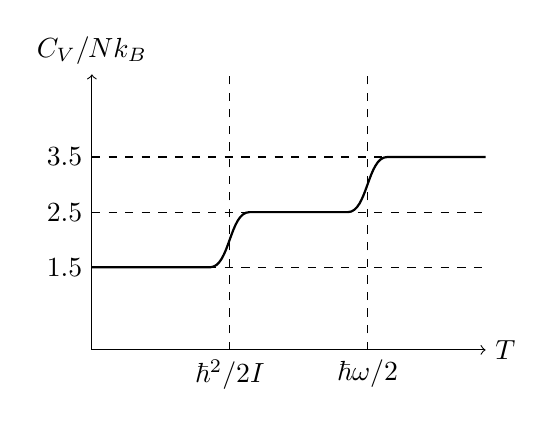
\begin{tikzpicture}[yscale=0.7]
    \draw [->] (0, 0) -- (5, 0) node [right] {$T$};
    \draw [->] (0, 0) -- (0, 5) node [above] {$C_V/Nk_B$};

    \draw [dashed] (1.75, 0) node [below] {$\hbar^2/2I$} -- +(0, 5);
    \draw [dashed] (3.5, 0) node [below] {$\hbar \omega/2$} -- +(0, 5);

    \draw [dashed] (0, 1.5) node [left] {$1.5$} -- +(5, 0);
    \draw [dashed] (0, 2.5) node [left] {$2.5$} -- +(5, 0);
    \draw [dashed] (0, 3.5) node [left] {$3.5$} -- +(5, 0);

    \draw [thick] (0, 1.5) -- (1.5, 1.5) .. controls (1.75, 1.5) and (1.75, 2.5) .. (2, 2.5) -- (3.25, 2.5) .. controls (3.5, 2.5) and (3.5, 3.5) .. (3.75, 3.5) -- (5, 3.5);
  \end{tikzpicture}
\end{center}
In quantum mechanics, the rotational eigenstates are discrete with eigenvalue
$$E_{\text{rot}}=\frac{\hbar^2}{2I}j(j+1),\quad j\in\mathbb{Z}^+\cup\{0\}$$
which has degeneracy $2j+1$. The single particle partition function is
$$Z_{\text{rot}}=\sum_{j=0}^\infty(2j+1)e^{-\beta\hbar^2j(j+1)/2I}$$
\begin{itemize}
    \item At high temperatures ($k_BT>>\frac{\hbar^2}{2I}$): we recover the classical result:
$$Z_{\text{rot}}\approx\int_0^\infty (2x+1)e^{-\beta\hbar^2x(x+1)/2I}dx=\frac{2Ik_BT}{\hbar^2}$$
The corresponding heat capacity is
$$C_{V,\text{rot}}=T\bigg(\frac{\partial S}{\partial T}\bigg)_V=-T\bigg(\frac{\partial^2F}{\partial T^2}\bigg)_V=k_BT\bigg(\frac{\partial^2T\log Z_{\text{rot}}^N}{\partial T^2}\bigg)_V=k_BTN\frac{\partial^2}{\partial T^2}T\log\frac{2Ik_BT}{\hbar^2}=k_BTN$$
\item At low temperatures ($k_BT<<\frac{\hbar^2}{2I}$):
 all states apart from $j=0$ effectively decouple and $Z_{\text{rot}}\approx1$, and thus the heat capacity vanishes.
 \end{itemize}
Similarly, the vibrational eigenstates are quantized with eigenvalue
$$E_{\text{vib}}=\hbar\omega(n+0.5),\quad n\in\mathbb{Z}^+\cup\{0\}$$
The single particle partition function is then
$$Z_{\text{vib}}=\sum_ne^{-\beta\hbar\omega(n+0.5)}=\frac{e^{-\beta\hbar\omega/2}}{1-e^{-\beta\hbar\omega}}=\frac{1}{2\sinh(\beta\hbar\omega/2)}$$
\begin{itemize}
    \item At high temperatures $k_BT>>\hbar\omega$: $Z_{\text{vib}}\approx\frac{1}{\beta\hbar\omega}$. The corresponding heat capacity is
  $$C_{V,\text{vib}}=T\bigg(\frac{\partial S}{\partial T}\bigg)_V=-T\bigg(\frac{\partial^2F}{\partial T^2}\bigg)_V=k_BT\bigg(\frac{\partial^2T\log Z_{\text{vib}}^N}{\partial T^2}\bigg)_V=k_BTN\frac{\partial^2}{\partial T^2}T\log\frac{k_BT}{\hbar\omega}=k_BTN$$  
  \item At low temperatures ($k_BT<<\hbar\omega$): $Z_{\text{vib}}\approx e^{-\beta\hbar\omega/2}$ and so the energy converges to the classical limit
  $$E_{\text{vib}}=-\frac{\partial}{\partial\beta}\log Z_{\text{vib}}\approx\frac{1}{2}\hbar\omega$$
  Similarly, the heat capacity vanishes as $-T\log Z_{\text{vib}}^N=0.5TN\hbar\omega/k_BT$ which is independent of temperature.
\end{itemize}
\end{remarks}
\begin{remarks}
The limit of a classical ideal gas is $N\lambda^3/V<<1$, i.e. the thermal de Broglie volumes associated with the particles do not clash. We can depart from this classical limit in several ways:
\begin{itemize}
    \item by increasing the density of particles $N/V$;
    \item by increasing the de Broglie wavelength $\lambda$, in turn achieved by either lowering the temperatures or by considering lighter particles.
\end{itemize}
In this case, their wavepackets will start interfering with each other and we are in the quantum regime. Equivalently, the quantum regime occurs when the occupancy of each of the energy levels becomes small and therefore the discreteness becomes relevant, i.e. reciprocal $k$-space condition. The average occupation of an accessible energy level is
$$\langle n\rangle=\frac{N}{4\pi k_{\text{max}}^3/3}\frac{(2\pi)^3}{V}$$
The crossover occur when $\langle n\rangle\sim 1$. $1/\lambda^3$ is sometimes called the quantum concentration $n_Q$.
\end{remarks}
\newpage
\section{Quantum Statistical Mechanics}
\subsection{Density of states}
The density of states appear a lot in this chapter when computing sums over states. Consider an ideal gas trapped in a box of volume $V=L^3$.
\subsubsection{Open Boundary Conditions}
If we assert the wavefunction must vanish at the walls of the box, then it must be standing waves. The eigenstates and eigenvalues are
$$\psi=\sqrt{\frac{8}{V}}\sin(k_xx)\sin(k_yy)\sin(k_zz),\quad E_{\mathbf{k}}=\frac{\hbar^2}{2m}(k_x^2+k_y^2+k_z^2)$$
In order to satisfy the boundary conditions, we need $\psi(x_i=0)=\psi(x_i=L_i)=0$, $k_i=\frac{n\pi}{L_i}$. The allowed values of the $\mathbf{k}$-vector form a lattice in $\mathbf{k}$-space, with volume per point $\Delta k_x\Delta k_y\Delta k_z=\frac{\pi^3}{V}$. The density of allowed $\mathbf{k}$-vectors will be the inverse of this, multiplied by the spin degeneracy factor $g_s$.
\subsubsection{Periodic Boundary conditions}
Now, since $\psi(x_i+L_i)=\psi(x_i)$, the eigenstates must be travelling waves $\psi=\frac{1}{\sqrt{V}}e^{i\mathbf{k}\cdot\mathbf{r}}$. The allowed values of the wavevector $\mathbf{k}$ again form a lattice, but now the spacing between lattice points is $2\pi/L_i$, giving a larger volume per lattice point $(2\pi)^3/V$ and a smaller density $g_sV/(2\pi)^3$. Since we count $\mathbf{k}$ from all eight octants of the 3D wavevector space, whereas for the open boundary conditions, states with wavevector $(\pm k_x,\pm k_y,\pm k_z)$ are actually the same, and so we have to limit our sums to one octant.
\subsubsection{Integral conversion}
For any macroscopic size box $(\lambda<<L)$, there are many states with $E_n\leq k_BT$ all of which contributes to the sum. Hence, we may approximate the discrete sum to an integral:
$$\sum_n\rightarrow\int d^3n=\frac{V}{(2\pi)^3}\int d^3k=\frac{4\pi V}{(2\pi)^3}\int_0^\infty k^2dk$$
It is thus easier to change variables to $dE=\frac{\hbar^2k}{m}dk$, so the density of states is
$$\int d^3n=\int g(E)dE,\quad g(E)=\frac{V}{4\pi^2}\bigg(\frac{2m}{\hbar^2}\bigg)^{3/2}E^{1/2}$$
where $g(E)dE$ counts the number of states with energy between $E$ and $E+dE$. On the other hand, for massless particles, the density of states is
$$g(E)=\frac{VE^2}{2\pi^2\hbar^3c^3}$$
\begin{remarks}
This conversion is necessary in order to compute the grand potential later. Recall that the full grand potential is summed over all energy states, i.e. $\Phi=\sum_k\Phi_k$. For a continuous non-relativistic gas in 3D, we can cast the discrete sum into an integral over available phase space.
$$\Phi=\sum_k\Phi_k=\int\Phi(E)\frac{d^3xd^3p}{(2\pi\hbar)^3}=\frac{V}{(2\pi\hbar)^3}\int^\infty_0 e^{-\beta(E-\mu)}4\pi p^2dp=\frac{V}{4\pi^2}\bigg(\frac{2m}{\hbar^2}\bigg)^{3/2}\int_0^\infty\sqrt{E}e^{-\beta(E-\mu)}dE$$
which gives $-k_BTVe^{\beta\mu}/\lambda^3$. 
\end{remarks}
\begin{eg}
Consider the partition function of a single particle of mass $m$ in a box of volume $V$,
$$Z_1=\sum_{k_x,k_y,k_z}e^{-\beta\varepsilon_{\mathbf{k}}}=\frac{V}{4\pi^2}\bigg(\frac{2m}{\hbar^2}\bigg)^{3/2}\int_0^\infty e^{-\beta\varepsilon}\sqrt{\varepsilon}d\varepsilon=\frac{V}{4\pi^2}\bigg(\frac{2mk_BT}{\hbar^2}\bigg)^{3/2}2\int_0^\infty e^{-x^2}x^2dx=\frac{V}{\lambda^3}$$
where we substituted $x^2=\varepsilon/k_BT$ and the integral is equal to $\sqrt{\pi}/4$. We have $n_Q(T)=1/\lambda^3$ to be the quantum concentration.
\end{eg}

\newpage
\subsection{Bosons and Fermions}
If particles are non-interacting and $\lambda\sim(V/N)^{1/3}$ at sufficiently low temperature, then we need to consider quantum statistics. Consider $N$ identical particles, which may be interacting with each other. Due to spin-statistics theorem, the quantum wavefunctions must obey the symmetry property (depending on the quantum statistics)
$$\Psi(\mathbf{x^1},...,\mathbf{x^i},...,\mathbf{x^j},...,\mathbf{x^N})=\pm\Psi(\mathbf{x^1},...,\mathbf{x^j},...,\mathbf{x^i},...,\mathbf{x^N})$$
Bosonic (integer spins) wavefunctions are even under exchange, whereas fermionic (half-integer spins) wavefunctions are odd under exchange. We can construct the basis of $N$-particle states $\Psi$ from independent 1-particle states $\{\psi^1, \psi^2,...\}$.  We do this by specifying the occupation numbers of $N$-particle states, constrained by the total number of particles $N$ being fixed, i.e. $\sum_\alpha n^\alpha=N$. The occupancy for bosons and fermions satisfy respectively $n^\alpha\in\mathbb{Z}^+\cup\{0\}$ and $n^\alpha\in\{0,1\}$. The latter is due to Pauli exclusion principle:
\begin{eg}[Pauli exclusion principle]
Consider the two-particle state constructed using $\psi^\alpha$ and $\psi^\beta$:
$$\Psi(\mathbf{x^1},\mathbf{x^2})=\psi^\alpha(\mathbf{x^1})\psi^\beta(\mathbf{x^2})\pm\psi^\alpha(\mathbf{x^2})\psi^\beta(\mathbf{x^1}),\quad\alpha\neq\beta$$
and $\Psi$ has the required symmetry in accordance to the spin-statistics theorem. Let the occupation numbers be $n^\alpha=1$ and $n^\beta =1$. If $\alpha=\beta$, $\Psi(\mathbf{x^1},\mathbf{x^2})=\psi^\alpha(\mathbf{x^1})\psi^\alpha(\mathbf{x^2})$. This is okay for bosons since $n^\alpha=2$ is allowed. But, no state with $n^\alpha=2$ is allowed for fermions.
\end{eg}
\begin{eg}
Consider two non-interacting quantum particles in a box, in states $|\mathbf{k_1}\rangle$ and $|\mathbf{k_2}\rangle$ with positions $\mathbf{r_1}$ and $\mathbf{r_2}$. Since the particles are indistinguishable, then the state $\Psi_{\mathbf{k_1},\mathbf{k_2}}(\mathbf{r_1},\mathbf{r_2})=e^{i\mathbf{k_1}\cdot\mathbf{r_1}}e^{i\mathbf{k_2}\cdot\mathbf{r_2}}$ is different from $\Psi_{\mathbf{k_2},\mathbf{k_1}}(\mathbf{r_1},\mathbf{r_2})=e^{i\mathbf{k_2}\cdot\mathbf{r_1}}e^{i\mathbf{k_1}\cdot\mathbf{r_2}}$. The wavefunction is
$$\Psi_{\mathbf{k_1},\mathbf{k_2}}(\mathbf{r_1},\mathbf{r_2})=\frac{1}{\sqrt{2}}\bigg(e^{i\mathbf{k_1}\cdot\mathbf{r_1}}e^{i\mathbf{k_2}\cdot\mathbf{r_2}}|s_1;s_2\rangle\pm e^{i\mathbf{k_2}\cdot\mathbf{r_1}}e^{i\mathbf{k_1}\cdot\mathbf{r_2}}|s_2;s_1\rangle\bigg)$$
where the plus sign refers to bosons, and the minus to fermions. The joint probability density $P_{\mathbf{k_1},\mathbf{k_2}}(\mathbf{r_1},\mathbf{r_2})$ for the state $\Psi_{\mathbf{k_1},\mathbf{k_2}}(\mathbf{r_1},\mathbf{r_2})$ of finding one particle at $\mathbf{r_1}$ and the other at $\mathbf{r_2}$ is
$$\frac{1}{2}(1+1\pm\delta_{s_1,s_2}(e^{-i\mathbf{k_1}\cdot(\mathbf{r_1}-\mathbf{r_2})}e^{-i\mathbf{k_2}\cdot(\mathbf{r_2}-\mathbf{r_1})}+e^{-i\mathbf{k_2}\cdot(\mathbf{r_1}-\mathbf{r_2})}e^{-i\mathbf{k_1}\cdot(\mathbf{r_2}-\mathbf{r_1})}))=(1\pm\delta_{s_1,s_2}\cos[(\mathbf{k_1}-\mathbf{k_2})\cdot(\mathbf{r_1}-\mathbf{r_2})])$$
which is called the pair-correlation function.
\end{eg}
Using the canonical ensemble framework, the partition function is
$$Z=\sum_{\{n_r\}}e^{-\beta n_rE_r}$$
where $n_r$ is the number of particles in the state $|r\rangle$, with $\sum_rn_r=N$ being the total number of particles. Imposing quantum statistics on this sum is tricky, so it is much easier if we use a chemical potential $\mu$ and allow the total number of particles $N$ to fluctuate, i.e. grand canonical ensemble framework. Treat each one-particle energy level to be in contact with a heat and particle reservoir of temperature $T$ and chemical potential $\mu$. There is no need to constrain total $E$ and $N$. Essentially, instead of treating the particles as independent thermodynamic systems, we treat the energy levels as independent thermodynamic systems, which contain particles and energy.
\begin{prop}
The macroscopic grand partition functions for bosons and fermions respectively are:
$$\mathcal{Z}_B=\frac{1}{1-e^{n\beta(\mu-E)}},\quad\mathcal{Z}_F=1+e^{n(\mu-E)\beta}$$
\end{prop}
\begin{proof}
For bosons, consider state $|r\rangle$ which may be populated by an arbitrary number of particles:
$$\mathcal{Z}^{\text{boson}}_r=\sum_{n_r}e^{-\beta n_r(E_r-\mu)}=\frac{1}{1-e^{-\beta(E_r-\mu)}},\quad n_r\in\mathbb{Z}^+\cup\{0\}$$
The sum does converge if $E_r-\mu>0$ which is true $\forall E_r$. But, the ground state is $E_0=0$, so we require $\mu<0$. On the other hand, for fermions, $|r\rangle$ is either occupied or not:
$$\mathcal{Z}^{\text{fermion}}_r=\sum_{n_r=0,1}e^{-\beta n_r(E_r-\mu)}=1+e^{-\beta(E_r-\mu)},\quad n_r\in\{0,1\}$$
There is no convergence issue in defining $\mathcal{Z}_r$, so there is no constraint on the sign of $\mu$.
\end{proof}
\begin{remarks}
We are summing over the number of particles in a given state, rather than summing over the states for a single particle. For photons or phonons (examples of bosons), since the particle number is not conserved, we have to set $\mu=0$ in order to use the grand canonical ensemble approach.
\end{remarks}
\begin{prop}
The Bose-Einstein distribution and Fermi-Dirac distribution are respectively
$$n_B(E)=\frac{1}{e^{\beta(E-\mu)}-1},\quad n_F(E)=\frac{1}{e^{\beta(E-\mu)}+1}$$
\end{prop}
\begin{proof}
Using results from the grand canonical ensemble: the mean occupation number for bosons and fermions are respectively:
$$n_B(E)=T\frac{\partial}{\partial\mu}\log \mathcal{Z}_B=-T\frac{\partial}{\partial\mu}\log(1-e^{(\mu-E)/T})=\frac{1}{e^{(E-\mu)/T}-1}$$
$$n_F(E)=T\frac{\partial}{\partial\mu}\log\mathcal{Z}_F=T\frac{\partial}{\partial\mu}(1+e^{n(\mu-E)/T})=\frac{e^{(\mu-E)/T}}{1+e^{(\mu-E)/T}}=\frac{1}{e^{(E-\mu)/T}+1}$$
\end{proof}
\begin{cor}
The quantum gas distributions reduce to the Maxwell-Boltzmann distribution.
\end{cor}
\begin{proof}
$$n\approx e^{-(E-\mu)/T},\quad \beta(E-\mu)>>1$$
\end{proof}
\begin{eg}
The Maxwell-Boltzmann probability distribution is obtained by
$$P(E)dE=\frac{1}{N}e^{-\beta(E-\mu)}g(E)dE=\frac{1}{N}\frac{V}{4\pi^2}\bigg(\frac{2m}{\hbar^2}\bigg)^{3/2}\frac{N\lambda^3}{V}e^{-\beta E}\sqrt{E}dE$$
which gives $P(v)dv=(\frac{m}{2\pi k_BT})^{3/2}e^{-\beta mv^2/2}4\pi v^2dv$, as expected.
\end{eg}
\begin{remarks}
As we will see later:
\begin{enumerate}
    \item The Bose-Einstein distribution diverges for $E=\mu$, and meaningless for $E<\mu$, where the reservoir floods the energy levels. Hence, we required $\mu<E_0$, where $E_0$ is the ground state energy. $\mu$ is determined by total particle number $N$, or vice-versa. $n_B$ decreases rapidly with $E$ if $T$ is small. We require $\mu\rightarrow E_0$ as $T\rightarrow 0$ for $N$ to remain fixed. Most particles then occupy ground state $E_0$ and the energy states similar in energy. 
    \item $n_F=0.5$ for $E=\mu$. The steepness of $n_F(E)$ increases as $T\rightarrow 0$. The levels are mostly filled for $E<\mu$ and empty for $E>\mu$. $\mu$ can take any value. The Fermi gas becomes degenerate at $T=0$. All states occupied up to energy $E_F=\mu$ (Fermi Energy) and empty above.
\end{enumerate}
\end{remarks}
\begin{prop}
Suppose we have a quasi-continuous density of 1-particle energy levels $g(E)$. The total particle number and total energy are respectively
$$N=\int_{E_{0}}^\infty\frac{g(E)dE}{e^{\beta(E-\mu)}\mp 1},\quad E=\int_{E_{0}}^\infty\frac{E g(E)dE}{e^{\beta(E-\mu)}\mp 1}$$
The negative branch is for bosons and positive branch is for fermions. 
\end{prop}
\begin{remarks}
In general, the two integrals have no closed form, but we can simplify it under certain regimes (as we will see later). For a gas of non-relativistic particles, $E=\frac{p^2}{2m}$, the density of states $g(E)$ is given to be
$$g(E)dE=g_s\frac{V}{(2\pi\hbar)^3}d^3p=\frac{g_sV4\pi p^2dp}{(2\pi\hbar)^3}=\frac{g_sV}{4\pi^2}\bigg(\frac{2m}{\hbar^2}\bigg)^{3/2}E^{1/2}dE:=K'E^{1/2}dE$$
where $g_s$ is the degeneracy of the particles.
\end{remarks} 
\begin{prop}
$PV=\frac{2}{3}E$ is true for bosons and fermions.
\end{prop}
\begin{proof}
$\Phi$ is extensive and a function of $T$, $\mu$ and $V$, i.e. $\Phi=Vf(T,\mu)$. Recall $P=-\frac{\partial\Phi}{\partial V}|_{T,\mu}=-f(T,\mu)$ and for boson/fermion gases, the grand potential $\Phi$ is
$$\Phi=-T\log\mathcal{Z}=-T\int g(E)\log(1\pm\xi e^{-E/T})dE=-TK'\int E^{1/2}\log(1\pm\xi e^{-E/T})dE$$
where $\xi=e^{\mu/T}$ is defined as the fugacity. Perform an integration by parts:
$$PV=-\Phi=T\log\mathcal{Z}=-TK'\int E^{1/2}\log(1\pm\xi e^{-\beta E})dE=K'\frac{2}{3}\int\frac{E^{3/2}dE}{\xi^{-1}e^{\beta E}\pm1}=\frac{2}{3}E$$
\end{proof}
\begin{defi}[Gamma function]
The Gamma function is defined to be
$$\Gamma(s)=\int_0^\infty t^{s-1}e^{-t}dt$$
with the familiar results:
$$\Gamma(n)=(n-1)!,\quad n\in\mathbb{Z}^+,\quad\Gamma(1/2)=\sqrt{\pi},\quad\Gamma(3/2)=\frac{\sqrt{\pi}}{2},\quad\Gamma(5/2)=\frac{3\sqrt{\pi}}{4}$$
\end{defi}
\begin{prop}
Let $x=\beta E$ and recall the thermal wavelength to be $\lambda=\sqrt{2\pi\hbar^2\beta/m}$. Then, $\frac{N}{V}$ and $\frac{P}{T}$ of fermions/bosons can be elegantly written as
$$\frac{N}{V}=\frac{g_s}{\lambda^3}f_{3/2}^{F/B}(\xi),\quad\frac{P}{T}=\frac{g_s}{\lambda^3}f_{5/2}^{F/B}(\xi)$$
where
$$f_\nu^F(\xi):=\frac{1}{\Gamma(\nu)}\int_0^\infty\frac{x^{\nu-1}}{\xi^{-1}e^x+1}dx,\quad f_\nu^B(\xi):=\frac{1}{\Gamma(\nu)}\int_0^\infty\frac{x^{\nu-1}}{\xi^{-1}e^x-1}dx$$
where $\Gamma(\nu)$ is the Gamma function.
\end{prop}
\begin{proof}
use the definition of $f_{3/2}^{F/B}(\xi)$, $f_{5/2}^{F/B}(\xi)$ and $\Gamma(3/2)=\sqrt{\pi}/2$, $\Gamma(5/2)=3\sqrt{\pi}/4$:
$$\frac{N}{V}=\int_0^\infty\frac{g(E)dE}{\xi^{-1}e^{\beta E}\mp 1}dE=\frac{g_s}{4\pi^2}\bigg(\frac{2m}{\hbar^2}\bigg)^{3/2}\int_0^\infty\frac{E^{1/2}dE}{\xi^{-1}e^{\beta E}\mp 1}=\frac{g_s}{4\pi^2}\bigg(\frac{2m}{\hbar^2\beta}\bigg)^{3/2}\int_0^\infty\frac{x^{1/2}dx}{\xi^{-1}e^x\mp 1}=\frac{g_s}{\lambda^3}f_{3/2}^{F/B}(\xi)$$
$$\frac{E}{V}=\int_0^\infty\frac{Eg(E)dE}{\xi^{-1}e^{\beta E}\mp 1}dE=\frac{g_s}{4\pi^2}\bigg(\frac{2m}{\hbar^2}\bigg)^{3/2}\int_0^\infty\frac{E^{3/2}dE}{\xi^{-1}e^{\beta E}\mp 1}=\frac{g_s}{4\pi^2}\bigg(\frac{2m}{\hbar^2\beta}\bigg)^{3/2}\frac{1}{\beta}\int_0^\infty\frac{x^{3/2}dx}{\xi^{-1}e^x\mp 1}=\frac{g_s}{\lambda^3}\frac{3}{2\beta}f_{5/2}^{F/B}(\xi)$$
But $PV=\frac{2}{3}E$ for quantum gases, so $\frac{P}{T}=\frac{g_s}{\lambda^3}\frac{2}{3}\frac{3}{2}f_{5/2}^{F/B}(\xi)$.
\end{proof}
\begin{remarks}
When $\xi=1$, we obtain the Riemann Zeta function
$$f_\nu^B(\xi=1)=\zeta(\nu)=\frac{1}{\Gamma(\nu)}\int_0^\infty\frac{x^{\nu-1}}{e^x-1}dx$$
In general, it is tricky to obtain analytical solutions, hence we shall only consider limiting cases.
\end{remarks}
\newpage
\subsection{Ideal Fermi Gas}
\begin{prop}
Fermionic particles repel in a low density fermionic gas.
\end{prop}
\begin{proof}
For low density, expand the Fermi-Dirac function for small $\xi$:
$$\frac{1}{\xi^{-1}e^x+1}=\xi e^{-x}(1-\xi e^{-x}+...)\implies f_\nu^F(\xi)=\frac{1}{\Gamma(\nu)}\int_0^\infty x^{\nu-1}(\xi e^{-x}-\xi^2e^{-2x}+...)d\xi=\xi-\frac{\xi^2}{2^\nu}+...$$
This gives
$$\frac{N}{V}=\frac{g_s}{\lambda^3}\bigg(\xi-\frac{\xi^2}{2^{3/2}}+\dots\bigg),\quad\frac{P}{T}=\frac{g_s}{\lambda^3}\bigg(\xi-\frac{\xi^2}{2^{5/2}}+\dots\bigg)$$
For dilute gas (low density) $\frac{N}{V}<<\frac{1}{\lambda^3}$, so $\xi<<1$. The leading result is $\frac{P}{T}=\frac{N}{V}$ as expected. The next leading term is obtained by eliminating $\xi$:
$$P=\frac{NT}{V}\bigg(1+\frac{1}{2^{5/2}}\frac{\lambda^3}{g_s}\frac{N}{V}\bigg)=\frac{NT}{V}\bigg(1+\frac{\pi^{3/2}\hbar^3}{2m^{3/2}T^{3/2}g_s}\frac{N}{V}\bigg)$$
The second Virial coefficient $B(T)$ (we will see later) is directly proportional to $T^{-3/2}$. This is small for large $T$, so $B(T)>0$, so pressure increase, i.e. fermions repel.
\end{proof}
\begin{prop}
Chemical potential is negative for a dilute fermionic gas.
\end{prop}
\begin{proof}
$\xi=e^{\mu/T}\approx\frac{\lambda^3N}{g_sV}<<1$ for dilute gas, hence $\mu\approx T\log\frac{\lambda^3N}{g_sV}<0$ and $n_F(\xi)$ is small for $\xi\geq0$. As $T$ decreases, $\lambda$ increases, so $\mu$ increases and becomes positive. 
\end{proof}
\begin{remarks}
To keep $N$ fixed, we have to adjust $\mu$ as the temperature changes. As the temperature is increased, the chemical potential (originally positive) shifts to lower values, and ultimately becomes negative.
\end{remarks}
\begin{eg}
$^3$He is well described by the ideal Fermi gas. It is gaseous down to $T=3$K. The atom has two protons, 1 neutron, 2 electrons, so it is a fermion of spin $\frac{1}{2}$. The mass $m$ is small, so $\lambda$ is relatively large for $T\sim 10$ K, i.e. quantum effects are significant.
\end{eg}
\begin{Note}[Fermi sphere]
For electronic gas, the degeneracy is $g_s=2$ since electrons have spin-$1/2$. At $T=0$, the Fermi-Dirac distribution is a step function, i.e. energy levels $E<\mu$ is filled while $E>\mu$ is empty. $\mu$ is called the Fermi energy $E_F$. Each fermion we add into the system settle into the lowest available energy state. These are successively filled until we run out of particles. the energy of the last filled state is called the Fermi energy, $E_F$ where $\mu$ at $T=0$ is $E_F$. Note that $\mu$ and $T$ are independent variables in the grand canonical ensemble.\\[5pt]
The energy states of the free particles are not localized in position space, but localized in momentum space. Successive fermions sit in states with ever-increasing momentum. Fermions fill out a ball in momentum space with the momentum of the final fermion called the Fermi momentum $k_F=\sqrt{2mE_F}/\hbar$. All states with wavevector $k\leq k_F$ are filled and are said to form the Fermi sphere.
\end{Note}
\begin{prop}
At $T=0$, electronic gas is degenerate and exhibit degeneracy pressure.
\end{prop}
\begin{proof}
For a fixed total particle number $N$ and $g_s=2$, the Fermi momentum satisfy
$$N=\frac{V}{\pi^2\hbar^3}\int_0^{p_F}p^2dp=\frac{Vp_F^3}{3\pi^2\hbar^3}$$
For non-relativistic particles, $E_F=\frac{p_F^2}{2m}$, so $N=\frac{V}{3\pi^2 h^3}(2mE_F)^{3/2}\implies E_F=\frac{\hbar^2}{2m}(3\pi^2)^{2/3}\frac{N^{2/3}}{V^{2/3}}$. The result for total particle number is also valid for highly relativistic particles, $E_F=cp_F$. The total energy is
$$E=\frac{V}{\pi^2\hbar^3}\int_0^{p_F}\frac{p^2}{2m}p^2dp=\frac{V}{10\pi^2m\hbar^3}p_F^5=\frac{V}{10\pi^2m\hbar^3}(2mE_F)^{5/2}\implies\frac{E}{N}=\frac{3}{10m}(2mE_F)=\frac{3}{5}E_F$$
The pressure is given by $$PV=\frac{2}{3}E=\frac{2}{5}NE_F\implies P=\frac{\hbar^2}{5m}(3\pi^2)^{2/3}\frac{N^{5/3}}{V^{5/3}}>0$$ 
This is the degeneracy pressure.
\end{proof}
\begin{remarks}
The repulsion of particles in Fermi gas produces pressure, even when $T=0$ due to Pauli Exclusion Principle. This effect is important for stabilizing white dwarf stars (degenerate electron gas) and neutron stars against gravitational collapse (i.e. becoming black hole).
\end{remarks}
\begin{prop}
For metals, the electronic contribution to the heat capacity dominates at low temperatures.
\end{prop}
\begin{proof}
The density of states $g(E)$ is independent of temperature $T$. For small $T$, the slope of $n_F$ at $E=\mu$ is $O(1/T)$ large. Between temperatures 0 and $T$, the number of particles that move is $O(g(E_F)k_BT)$. As $g(E)$ is approximately constant around $E_F$, $\mu$ does not need to change much to keep $N$ fixed. The increase in total energy between temperatures 0 and $T$ is $O(T^2g(E_F)k_B^2)$, i.e. $E(T)=E(0)+O(g(E_F)T^2k_B^2)\implies C=O(g(E_F)Tk_B^2)$. 
\end{proof}
\begin{center}
  \begin{tikzpicture}
    \draw [->] (0, 0) -- (5, 0) node [right] {$E$};
    \draw [->] (0, 0) -- (0, 3) node [above] {$n_F(E)$};

    \draw [thick](0, 2) -- (2, 2) -- (2, 0) node [below] {$E_f$} -- (4.9, 0);
  \end{tikzpicture}
  \begin{tikzpicture}
    \draw [->] (0, 0) -- (5, 0) node [right] {$E$};
    \draw [->] (0, 0) -- (0, 3) node [above] {$n_F(E)$};

    \draw [thick] (0, 2) -- (1.8, 2) .. controls (2, 2) and (2, 0) .. (2.2, 0) -- (4.9, 0);

    \node [below] at (2, 0) {$E_f$};
    \draw [decoration={markings, mark=at position 0 with {\arrowreversed{latex'}}, mark=at position 1 with {\arrow{latex'}}}, postaction={decorate}] (1.8, 2.2) -- (2.2, 2.2) node [pos=0.5, above] {$k_BT$};
  \end{tikzpicture}
\end{center}
\begin{remarks}\leavevmode
\begin{enumerate}
\item A more rigorous proof to the above is via the Sommerfield expansion. 
$$\int_0^\infty\frac{g(E)dE}{e^{\beta(E-\mu)}+1}\approx\int_0^{E_F}g(E)dE+\frac{\pi^2}{6}k_B^2T^2g'(E_F)+\frac{7\pi^4}{360}k_B^4T^4g^{(3)}(E_F)+\dots$$
To get the grand potential $\Phi$ to second order in $k_BT$, we substitute $g(E)=E^{3/2}$ to obtain
$$\Phi(T)=\Phi(0)-\frac{Vk_B^2T^2}{12}\bigg(\frac{2m}{\hbar^2}\bigg)^{3/2}E_F^{1/2}$$
and hence the heat capacity at constant volume is
$$C_V=T\bigg(\frac{\partial S}{\partial T}\bigg)_{V,\mu}=-T\bigg(\frac{\partial^2\Phi}{\partial T^2}\bigg)_{V,\mu}=T\frac{\partial}{\partial T}\frac{k_B^2T}{3}\frac{V}{2}\bigg(\frac{2m}{\hbar^2}\bigg)^{3/2}\sqrt{E_F}=\frac{\pi^2}{3}g(E_F)k_B^2T$$
\item In solid metal, the contributions to $C$ are $O(T)$ from non-degenerate electrons and $O(T^2)$ from lattice vibrations. The electronic contribution to the heat capacity dominates at low temperatures. The Fermi temperature $T_F$ is very large for metals, typically 50,000 K.
\end{enumerate}
\end{remarks}
\newpage
\subsection{Ideal Bose Gas}
\begin{prop}
Bosonic particles attract in a low density bosonic gas.
\end{prop}
\begin{proof}
Set $g_s=1$. For low density, expand Bose-Einstein function for small $\xi$:
$$\frac{N}{V}=\frac{1}{\lambda^3}f_{3/2}^B(\xi)=\frac{1}{\lambda^3}\bigg(\xi+\frac{\xi^2}{2^{3/2}}+...\bigg),\quad \frac{P}{T}=\frac{1}{\lambda^3}f_{5/2}^B(\xi)=\frac{1}{\lambda^3}\bigg(\xi+\frac{\xi^2}{2^{5/2}}+...\bigg)$$
At low density, $\xi<<1$. Eliminating $\xi$ gives
$$P=\frac{NT}{V}\bigg(1-\frac{\lambda^3}{2^{5/2}}\frac{N}{V}+...\bigg)$$
The second Virial coefficient (as we will see later) $B(T)=O(T^{-3/2})$ and is negative, i.e. Bosons are attractive.
\end{proof}
\begin{defi}[Bose-Einstein Condensation]
Bose-Einstein condensation is a condensate in momentum/energy space where a macroscopic number of particles occupy the ground state.
\end{defi}
\begin{prop}
At a critical temperature $T_c$, we will obtain Bose-Einstein condensation.
\end{prop}
\begin{proof}
Recall $\frac{N}{V}=\frac{1}{\lambda^3}f_{3/2}^B(\xi)$. As $T$ decreases, $\frac{1}{\lambda^3}$ decreases, so $\xi$ must increase to keep $\frac{N}{V}$ fixed. After $\xi$ reaches to 1, this equation breaks down (see $f_\nu^B$ integral). The critical temperature $T_c$ is given by
$$\frac{N}{V}=\frac{1}{[\lambda(T=T_c)]^3}f_{3/2}^B(1)=\bigg(\frac{mk_BT_c}{2\pi\hbar^2}\bigg)^{3/2}\zeta(1.5)\implies T_c=\frac{2\pi\hbar^2}{k_Bm}\bigg(\frac{1}{\xi(1.5)}\frac{N}{V}\bigg)^{2/3}$$
where $\zeta(1.5)=2.612$. $T_c$ is called the Bose-Einstein Condensation temperature, related to the number density $\frac{N}{V}$. Naively, we see that as we reduce $T$ below $T_c$, the number of particles $N$ should decrease. This is erroneous since in approximating the finite sum $\sum_k\rightarrow\frac{V(2m)^{3/2}}{4\pi^2\hbar^2}\int E^{1/2}dE$, $E=0$ does not contribute to the integral. The `missing' states have $E=0$ which does not contribute to the integral. Using the Bose-Einstein distribution, the ground state occupancy is predicted to be
$$n_B(E=0)=\frac{1}{\xi^{-1}-1}$$
which diverges at $\xi=0$. As $T\rightarrow T_c$ from above, one crudely approximate by setting $\xi\approx1-(1/N)$ so $n_B=O(N)$, i.e. the ground state have macroscopic occupation. 
\end{proof}
\begin{remarks}\leavevmode
\begin{enumerate}
    \item At low temperatures, $\mu\approx 0$ and it becomes more negative as temperature increases. $\mu\geq0$ cannot be true, otherwise the occupation number at $E=\mu$ would become infinite, contradicting our assumption on fixed total $N$.
    \item The correct approach for $T\leq T_c$: separate ground state from the quasi-continuum of positive energy states. Then,
$$\frac{N}{V}=\frac{N_0}{V}+\frac{1}{\lambda^3}f_{3/2}^B(\xi=1)\implies\frac{N_0}{V}=\frac{N}{V}-2.612\bigg(\frac{mk_BT}{2\pi\hbar^2}\bigg)^{3/2}\implies\frac{N_0}{N}=1-\bigg(\frac{T}{T_c}\bigg)^{3/2}$$
This gives us the fraction of particles in the ground state. At $T=0$, all particles will be in the ground state.
\begin{center}
  \begin{tikzpicture}
    \draw [->] (0, 0) -- (3, 0) node [right] {$T$};
    \draw [->] (0, 0) -- (0, 2) node [above] {$N_0/N$};
    \draw (0, 1) node [left] {1};
    \draw (1, 0) node [below] {$T_c$};
    \draw [thick, domain=0:1] plot [smooth] (\x, {1-\x^(3/2)});
  \end{tikzpicture}
\end{center}
\item The pressure is given by
$$\frac{P}{T}=\frac{g_s}{\lambda^3}f_{5/2}^B(\xi)=\frac{g_s}{\lambda^3}\zeta(5/2)$$
so $P$ is directly proportional to $T^{5/2}$ for $T\leq T_c$. Earlier, $PV=\frac{2}{3}E$, so $E$ is directly proportional to $VT^{5/2}$. This is true for $T< T_c$ and $\xi\approx 1$. 
\item At low temperatures and below $T_c$, set $\mu=0$, we have
$$U=\frac{2Vk_BT}{\sqrt{\pi}\lambda^3}\int_0^\infty\frac{x^{3/2}dx}{e^x-1}\approx\frac{2V}{\lambda^3}k_BT\propto T^{5/2}$$
and so the heat capacity is
$$C_V=\frac{\partial E}{\partial T}|_V=\frac{5}{2}\frac{k_BV}{\sqrt{2}\lambda^3}\propto T^{3/2}$$
For large $T$, estimate $C_V$ using virial expansion (see later):
$$E=\frac{3}{2}PV=\frac{3}{2}NT\bigg(1-O\bigg(\frac{N}{V}\frac{1}{T^{3/2}}\bigg)\bigg)\implies C_V=\frac{\partial E}{\partial T}\bigg|_V=\frac{3}{2}N\bigg(1+O\bigg(\frac{N}{V}\frac{1}{T^{3/2}}\bigg)\bigg)$$
\begin{center}
  \begin{tikzpicture}
    \draw [->] (0, 0) -- (6, 0) node [right] {$T$};
    \draw [->] (0, 0) -- (0, 4) node [above] {$C_V/N$};

    \draw [thick, domain=0.001:2] plot [smooth] (\x, {\x^(3/2)});

    \draw [dashed] (2, 0) node [below] {$T_c$} -- (2, 2.83);

    \draw [thick] (2, 2.83) .. controls (2.5, 2) .. (6, 2);

    \draw [dashed] (0, 2) node [left] {$\frac{3}{2}$} -- (6, 2);
  \end{tikzpicture}
\end{center}
\end{enumerate}
\item $C_V$ is continuous but have a discontinuous derivative at $T=T_c$. We call this a phase transition, and that $T_c$ depends on $\frac{N}{V}$.
\end{remarks}
\begin{eg}
$^4$He undergoes transition from normal liquid to a superfluid (related to Bose Einstein condensation, but interactions are really quite strong). Using the density of normal liquid at pressure 1 atm, we predict the Bose Einstein transition temperature $T_c=3.13$ K. Experimentally, we see a discontinuity in $C_V$ at $T=2.19$ K. The experimental measurements show a `$\lambda$' transition at $T_c$. This is because in our calculations, interactions are not accounted for. Better examples of BEC are dilute gases of heavy atoms in harmonic traps, like Rubidium-87 which have a $T_c\sim 10^{-7}$ K with a macroscopic occupation of $N\sim10^4$ to $10^7$, i.e. density of $2.5\times10^{12}$ atoms per cubic centimetres. 
\end{eg}
\begin{Note}
The exact description of interacting particles is very difficult. Commonly, we can take a system which is close to its ground state and subject it to a weak external influence, and are interested in the small changes to the system caused by the external influence. These are the excited states or excitations of the system, which interact only weakly with one another. We thus approximate them as non-interacting ideal gases. We interpret their low temperature properties in terms of approximate normal modes, or `elementary excitations'. These are characterized by the zero rest mass (infinite de Broglie wavelength, hence always in the quantum regime) and are always bosons (most have no spins).
\end{Note}
\begin{eg}[Spin waves]
The elementary excitations of a ferromagnetic systems, in which the size of the moments is fixed, are `spin waves'. The simplest dispersion relation is $E_k\propto k^2$. The result will be $C\propto T^{3/2}$, which agrees with experimental measurements.
\end{eg}
Below, we consider two other examples: photons and phonons.
\newpage
\subsection{Blackbody radiation}
\begin{defi}[Blackbody radiation]
Blackbody radiation can be thought of as an ideal gas of photons, with integer angular momentum and obey Bose statistics. To come into equilibrium, they have to interact with a reservoir, which is taken to be the walls of the blackbody cavity.
\end{defi}
\begin{prop}
The chemical potential of blackbody radiation is zero.
\end{prop}
\begin{proof}
Thermal equilibrium is reached by absorption and emission of photons by the walls, so we cannot take $N$, the number of photons in the gas, to be constant. $\mu$ is obtained by minimizing the Helmholtz free energy, with respect to the variations in the average number of photons, i.e.
$$\bigg(\frac{\partial F}{\partial N}\bigg)_{T,V}=0$$
But this is actually $\mu$ by definition of free energy. In this case, the grand potential and the free energy is the same.
\end{proof}
\begin{prop}
The Planck distribution $E(\omega)$ is given by
$$E=\int_0^\infty E(\omega)d\omega,\quad E(\omega)=\frac{V\hbar}{\pi^2c^3}\frac{\omega^3}{e^{\beta\hbar\omega}-1}$$
\end{prop}
\begin{proof}
Consider electromagnetic radiation filling a volume $V=L^3$ at temperature $T$. The radiation modes are $\mathbf{A}e^{i(\mathbf{k}\cdot\mathbf{x}-\omega t)}$ with $\omega=c|\mathbf{k}|$. Again, enforce periodic boundary conditions are $k_x=\frac{2\pi n_x}{L}$, etc. There are two transverse polarization states which are the two directions transverse to the direction of propagation, so the degeneracy $g_s=2$. Hence, the density of modes in $\mathbf{k}$-space is $2\frac{V}{(2\pi)^3}$. The number of modes between $k$ and $k+dk$ is 
$$g(k)dk=2\frac{V}{(2\pi)^3}4\pi k^2dk=\frac{Vk^2}{\pi^2}dk$$
Correspondingly, the number of modes between $\omega$ and $\omega+d\omega$ is 
$$g(\omega)d\omega=\frac{V\omega^2}{\pi^2c^3}d\omega$$
where we used $\omega=ck$, i.e. relativistic. We start by summing photons with a definite frequency $\omega$. A state with $N$ such photons has energy $E=N\hbar\omega$.
$$Z_\omega=\sum_{N=0}^\infty e^{-\beta N\hbar\omega}=\frac{1}{1-e^{-\beta\hbar\omega}}$$
Sum over all possible frequencies:
$$\ln Z=\int_0^\infty g(\omega)\ln Z_\omega d\omega=-\frac{V}{\pi^2c^3}\int_0^\infty\omega^2\ln(1-e^{-\beta\hbar\omega})d\omega$$
Using the result from the canonical ensemble, the energy is
$$E=-\frac{\partial}{\partial\beta}\log Z=\frac{V\hbar}{\pi^2c^3}\int_0^\infty\frac{\omega^3d\omega}{e^{\beta\hbar\omega}-1}$$
Result follows by $E=\int_0^\infty E(\omega)d\omega$.
\end{proof}
\begin{cor}[Wien's displacement law]
The Planck distribution peaks at a frequency $\omega_{\text{max}}=\xi T/\hbar$ where $\xi$ satisfies $3-\xi=3e^{-\xi}$.
\end{cor}
\begin{proof}
Find maximum for the Planck distribution $E(\omega)$.
\end{proof}
\begin{prop}[Stefan-Boltzmann Law]
The energy flux is given by $\sigma T^4$.
\end{prop}
\begin{proof}
Substitute $x=\beta\hbar\omega$ in the $E$ integral:
$$E=\frac{V}{\pi^2c^3}\frac{T^4}{\hbar^3}\int_0^\infty\frac{x^3dx}{e^x-1}=\frac{VT^4}{\pi^2c^3\hbar^3}\frac{\pi^4}{15}$$
The energy flux is the rate of transfer of energy and can be shown to be $\frac{E}{V}\frac{c}{4}$. The flux of photons is obtained from
$$\frac{1}{4\pi}\int_0^{2\pi}\int_0^{\pi/2}c\cos\theta (\sin\theta d\theta) d\phi=\frac{c}{4}$$
where we consider photons travelling perpendicularly away from the object. The result follows.
\end{proof}
\begin{prop}
The equation of state of the photon gas is
$$P=\frac{1}{3}\frac{E}{V}$$
\end{prop}
\begin{proof}
The free energy of a canonical ensemble is
\begin{align}
F&=-T\log Z\nonumber\\&=\frac{VT}{\pi^2c^3}\int_0^\infty\omega^2\log(1-e^{-\beta\hbar\omega})d\omega\nonumber\\&=-\frac{V\hbar}{3\pi^2c^3}\int_0^\infty\frac{\omega^3e^{-\beta\hbar\omega}}{1-e^{-\beta\hbar\omega}}d\omega\nonumber\\&=-\frac{V\hbar}{3\pi^2c^3\beta^4\hbar^4}\int_0^\infty\frac{x^3}{e^x-1}dx\nonumber\\&=-\frac{V\pi^2T^4}{45\hbar^3c^3}\nonumber
\end{align}
The pressure is then
$$P=-\bigg(\frac{\partial F}{\partial V}\bigg)_T=\frac{E}{3V}$$
or sometimes written as $4\sigma T^4/3c$. This is the radiation pressure. 
\end{proof}
\begin{remarks}\leavevmode
\begin{enumerate}
\item Alternatively, the equation of state can be worked out using the following argument: We have $k=\frac{\pi^2}{15\hbar^3c^3}$. Write $E=kVT^4$. At constant $V$,
$$dE=4kVT^3dT=TdS=TVf'(T)dT$$
where $S=Vf(T)$ is extensive. We must have $f'(T)=4kT^2$ and so $f(T)=\frac{4}{3}kT^3$ since $S(T=0)=0$ by Third Law. The entropy of blackbody radiation is $S=\frac{4}{3}kVT^3$. Now express $E$ in terms of $S$ and $V$. We have $E=kV(\frac{4}{3}kV)^{-4/3}S^{4/3}$ which is directly proportional to $V^{-1/3}$. The pressure is 
$$P=-\frac{\partial E}{\partial V}\bigg|_S\implies PV=\frac{1}{3}E$$
Hence, in an adiabatic change (slowly enlarge box with radiation inside), $PV^{4/3}$ is a constant and $TV^{1/3}$ is another constant. Hence, radiation cools as box expands.
\item We can also work out
$$S=-\bigg(\frac{\partial F}{\partial T}\bigg)_V=\frac{16V\sigma}{3c}T^3,\quad C_V=\bigg(\frac{\partial E}{\partial T}\bigg)_V=\frac{16V\sigma}{c}T^3$$
\item In the classical limit $\hbar\omega<<T$, we have
$$\frac{1}{e^{\beta\hbar\omega}-1}\approx\frac{1}{\beta\hbar\omega}\implies E(\omega)\approx\frac{V\omega^2T}{\pi^2c^3}$$
which is the Rayleigh-Jeans law for the classical distribution of radiation. This leads to the Ultraviolet catastrophe since $\int_0^\infty E(\omega)d\omega$ diverges.
\item Alternatively, we may compute the total number and energy of photon gas respectively to be:
$$N=\frac{V}{\pi^2c^3}\int_0^\infty\frac{\omega^2d\omega}{e^{\hbar\omega/T}-1}=\frac{VT^3}{\pi^2\hbar^3c^3}\int_0^\infty\frac{x^2dx}{e^x-1}=\frac{2\zeta(3)T^3}{\pi^2\hbar^3c^3}V$$
$$E=\frac{V\hbar}{\pi^2c^3}\int_0^\infty\frac{\omega^3d\omega}{e^{\hbar\omega/T}-1}=\frac{VT^4}{\pi^2\hbar^3c^3}\int_0^\infty\frac{x^3dx}{e^x-1}=\frac{\pi^2T^4}{15\hbar^3c^3}V$$
where $\zeta(\nu)=\int_0^\infty\frac{x^{\nu-1}}{e^x-1}dx$, is the Riemann zeta function such that $\zeta(3)\approx 0.244$ and $\zeta(4)=\frac{\pi^4}{15}$.
\end{enumerate}
\end{remarks}
\subsection{Vibrational Energy of Solids}
\begin{defi}[Phonons]
The atoms of a solid interact very strongly with one another. Sound waves in solids come in discrete packets, called phonons.
\end{defi}
Consider an atomic crystal with $N$ atoms such that the vibrational modes are $\mathbf{A}e^{i(\mathbf{k}\cdot\mathbf{x}-\omega t)}$. The degeneracy is 3, i.e. $g_s=3$, with a total of one longitudinal and two transverse polarizations. The frequency $\omega$ is related to $\hbar|\mathbf{k}|$ in some complicated way. At long wavelengths, we have sound waves $\omega=v_s|\mathbf{k}|$ where $v_s$ is an effective velocity ($3/v_s^3=(1/v_L^3)+(2/v_T^3)$ where $v_L$ and $v_T$ are longitudinal and transverse velocities respectively).  Assume small speed $v_s$, the number of modes between frequencies $\omega$ and $\omega+d\omega$ is
$$g(\omega)d\omega=\frac{3V\omega^2d\omega}{2\pi^2v_s^2}$$
Each mode of frequency $\omega$ can be excited to any $n$-phonon state of energy $n\hbar\omega$. 
\begin{prop}
There is an upper frequency limit, known as the Debye frequency, with $\omega_D=(\frac{6\pi^2N}{V})^{1/3}c_s$.
\end{prop}
\begin{proof}
Sound waves cannot propagate through the solid if the wavelength of sound is smaller than the atomic spacing, so we have have $\lambda=\frac{2\pi c_s}{\omega}<L$, where $L$ is the length of the crystal. Since there is three directions of motion for each of the $N$ atoms, then 
$$3N=\int_0^{\omega_D}g(\omega)d\omega=\frac{V\omega_D^3}{2\pi^2c_s^3}$$
\end{proof}
\begin{defi}[Debye temperature]
The Debye temperature is the temperature at which the highest frequency phonon starts to become excited, i.e. $T_D=\hbar\omega_D$.
\end{defi}
\begin{prop}
The vibrational heat capacity scales with $T^3$ for low temperatures and is a constant of $3N$ for high temperatures. The latter is called Dulong-Petit law.
\end{prop}
\begin{proof}
Since the number of phonons is not conserved, we perform a similar procedure as that of photons.
$$\log Z_{\text{phonon}}=\int_0^{\omega_D}g(\omega)\log Z_\omega d\omega,\quad Z_\omega=\frac{1}{1-e^{-\beta\hbar\omega}}$$
The energy is then
$$E=\int_0^{\omega_D}\frac{\hbar\omega g(\omega)}{e^{\beta\hbar\omega}-1}d\omega=\frac{3V\hbar}{2\pi^2c_s^3}\int_0^{\omega_D}\frac{\omega^3d\omega}{e^{\beta\hbar\omega}-1}=\frac{3Vk_BT^4}{2\pi^2\hbar^3c_s^3}\int_0^{T_D/T}\frac{x^3}{e^x-1}dx$$
where we substituted $x=\beta\hbar\omega$. This however has no analytical solution. For low temperatures, $T<<T_D$, the upper integration limit approaches infinity. Like before, the integral is thus $\frac{\pi^4}{15}$. The heat capacity is then
$$C_V=\bigg(\frac{\partial E}{\partial T}\bigg)_V=\frac{2\pi^2VT^3}{5\hbar^3c_s^3}=\frac{12\pi^4Nk_B}{5T_D^3}T^3$$
For high temperatures, $T>>T_D$, we Taylor expand the integrand,
$$\int_0^{T_D/T}\frac{x^3}{e^x-1}dx\approx\int_0^{T_D/T}x^2+...~dx=\frac{T_D^3}{3T^3}+...\implies C_V=\frac{Vk_BT_D^3}{2\pi^2\hbar^3c_s^3}=3Nk_B$$
where we invoked the definition of Debye temperature, i.e. $T_D^3=\hbar^3\omega_D^3=\hbar^3(3N)2\pi^2c_s^3/V$
\end{proof}
\newpage
\section{Classical Interacting Systems}
\subsection{Mixing and Phase Separation}
\subsection{Phase Transitions}
\subsection{Landau Theory of Phase Transitions}
\subsection{Critical Exponents and Universality}
How about ising model, lattice gas, broken symmetry and range of correlations, mean field theory, variational treatment of mean field theory, renormalization group theory


\newpage
\section{Fluctuations in Equilibrium}
\subsection{Fluctuations}
\subsection{Connection with Thermodynamics}
\subsection{Near Critical Points}

how about fluctuation-dissipation theorem, response functions, absorption, friction and Langevin equation

\newpage
\section{Stochastic Physics}
\subsection{Brownian Motion}
\subsection{Diffusion of Free and Confined Particles}
\subsection{Damped Harmonic Oscillator}
\subsection{Diffusion in External Potentials}

\appendix
\newpage
\bibliographystyle{unsrt}
\bibliography{reference.bib}
\end{document}